% Options for packages loaded elsewhere
\PassOptionsToPackage{unicode}{hyperref}
\PassOptionsToPackage{hyphens}{url}
\PassOptionsToPackage{dvipsnames,svgnames,x11names}{xcolor}
%
\documentclass[
  letterpaper,
  DIV=11,
  numbers=noendperiod]{scrreprt}

\usepackage{amsmath,amssymb}
\usepackage{iftex}
\ifPDFTeX
  \usepackage[T1]{fontenc}
  \usepackage[utf8]{inputenc}
  \usepackage{textcomp} % provide euro and other symbols
\else % if luatex or xetex
  \usepackage{unicode-math}
  \defaultfontfeatures{Scale=MatchLowercase}
  \defaultfontfeatures[\rmfamily]{Ligatures=TeX,Scale=1}
\fi
\usepackage{lmodern}
\ifPDFTeX\else  
    % xetex/luatex font selection
\fi
% Use upquote if available, for straight quotes in verbatim environments
\IfFileExists{upquote.sty}{\usepackage{upquote}}{}
\IfFileExists{microtype.sty}{% use microtype if available
  \usepackage[]{microtype}
  \UseMicrotypeSet[protrusion]{basicmath} % disable protrusion for tt fonts
}{}
\makeatletter
\@ifundefined{KOMAClassName}{% if non-KOMA class
  \IfFileExists{parskip.sty}{%
    \usepackage{parskip}
  }{% else
    \setlength{\parindent}{0pt}
    \setlength{\parskip}{6pt plus 2pt minus 1pt}}
}{% if KOMA class
  \KOMAoptions{parskip=half}}
\makeatother
\usepackage{xcolor}
\setlength{\emergencystretch}{3em} % prevent overfull lines
\setcounter{secnumdepth}{5}
% Make \paragraph and \subparagraph free-standing
\makeatletter
\ifx\paragraph\undefined\else
  \let\oldparagraph\paragraph
  \renewcommand{\paragraph}{
    \@ifstar
      \xxxParagraphStar
      \xxxParagraphNoStar
  }
  \newcommand{\xxxParagraphStar}[1]{\oldparagraph*{#1}\mbox{}}
  \newcommand{\xxxParagraphNoStar}[1]{\oldparagraph{#1}\mbox{}}
\fi
\ifx\subparagraph\undefined\else
  \let\oldsubparagraph\subparagraph
  \renewcommand{\subparagraph}{
    \@ifstar
      \xxxSubParagraphStar
      \xxxSubParagraphNoStar
  }
  \newcommand{\xxxSubParagraphStar}[1]{\oldsubparagraph*{#1}\mbox{}}
  \newcommand{\xxxSubParagraphNoStar}[1]{\oldsubparagraph{#1}\mbox{}}
\fi
\makeatother

\usepackage{color}
\usepackage{fancyvrb}
\newcommand{\VerbBar}{|}
\newcommand{\VERB}{\Verb[commandchars=\\\{\}]}
\DefineVerbatimEnvironment{Highlighting}{Verbatim}{commandchars=\\\{\}}
% Add ',fontsize=\small' for more characters per line
\usepackage{framed}
\definecolor{shadecolor}{RGB}{241,243,245}
\newenvironment{Shaded}{\begin{snugshade}}{\end{snugshade}}
\newcommand{\AlertTok}[1]{\textcolor[rgb]{0.68,0.00,0.00}{#1}}
\newcommand{\AnnotationTok}[1]{\textcolor[rgb]{0.37,0.37,0.37}{#1}}
\newcommand{\AttributeTok}[1]{\textcolor[rgb]{0.40,0.45,0.13}{#1}}
\newcommand{\BaseNTok}[1]{\textcolor[rgb]{0.68,0.00,0.00}{#1}}
\newcommand{\BuiltInTok}[1]{\textcolor[rgb]{0.00,0.23,0.31}{#1}}
\newcommand{\CharTok}[1]{\textcolor[rgb]{0.13,0.47,0.30}{#1}}
\newcommand{\CommentTok}[1]{\textcolor[rgb]{0.37,0.37,0.37}{#1}}
\newcommand{\CommentVarTok}[1]{\textcolor[rgb]{0.37,0.37,0.37}{\textit{#1}}}
\newcommand{\ConstantTok}[1]{\textcolor[rgb]{0.56,0.35,0.01}{#1}}
\newcommand{\ControlFlowTok}[1]{\textcolor[rgb]{0.00,0.23,0.31}{\textbf{#1}}}
\newcommand{\DataTypeTok}[1]{\textcolor[rgb]{0.68,0.00,0.00}{#1}}
\newcommand{\DecValTok}[1]{\textcolor[rgb]{0.68,0.00,0.00}{#1}}
\newcommand{\DocumentationTok}[1]{\textcolor[rgb]{0.37,0.37,0.37}{\textit{#1}}}
\newcommand{\ErrorTok}[1]{\textcolor[rgb]{0.68,0.00,0.00}{#1}}
\newcommand{\ExtensionTok}[1]{\textcolor[rgb]{0.00,0.23,0.31}{#1}}
\newcommand{\FloatTok}[1]{\textcolor[rgb]{0.68,0.00,0.00}{#1}}
\newcommand{\FunctionTok}[1]{\textcolor[rgb]{0.28,0.35,0.67}{#1}}
\newcommand{\ImportTok}[1]{\textcolor[rgb]{0.00,0.46,0.62}{#1}}
\newcommand{\InformationTok}[1]{\textcolor[rgb]{0.37,0.37,0.37}{#1}}
\newcommand{\KeywordTok}[1]{\textcolor[rgb]{0.00,0.23,0.31}{\textbf{#1}}}
\newcommand{\NormalTok}[1]{\textcolor[rgb]{0.00,0.23,0.31}{#1}}
\newcommand{\OperatorTok}[1]{\textcolor[rgb]{0.37,0.37,0.37}{#1}}
\newcommand{\OtherTok}[1]{\textcolor[rgb]{0.00,0.23,0.31}{#1}}
\newcommand{\PreprocessorTok}[1]{\textcolor[rgb]{0.68,0.00,0.00}{#1}}
\newcommand{\RegionMarkerTok}[1]{\textcolor[rgb]{0.00,0.23,0.31}{#1}}
\newcommand{\SpecialCharTok}[1]{\textcolor[rgb]{0.37,0.37,0.37}{#1}}
\newcommand{\SpecialStringTok}[1]{\textcolor[rgb]{0.13,0.47,0.30}{#1}}
\newcommand{\StringTok}[1]{\textcolor[rgb]{0.13,0.47,0.30}{#1}}
\newcommand{\VariableTok}[1]{\textcolor[rgb]{0.07,0.07,0.07}{#1}}
\newcommand{\VerbatimStringTok}[1]{\textcolor[rgb]{0.13,0.47,0.30}{#1}}
\newcommand{\WarningTok}[1]{\textcolor[rgb]{0.37,0.37,0.37}{\textit{#1}}}

\providecommand{\tightlist}{%
  \setlength{\itemsep}{0pt}\setlength{\parskip}{0pt}}\usepackage{longtable,booktabs,array}
\usepackage{calc} % for calculating minipage widths
% Correct order of tables after \paragraph or \subparagraph
\usepackage{etoolbox}
\makeatletter
\patchcmd\longtable{\par}{\if@noskipsec\mbox{}\fi\par}{}{}
\makeatother
% Allow footnotes in longtable head/foot
\IfFileExists{footnotehyper.sty}{\usepackage{footnotehyper}}{\usepackage{footnote}}
\makesavenoteenv{longtable}
\usepackage{graphicx}
\makeatletter
\newsavebox\pandoc@box
\newcommand*\pandocbounded[1]{% scales image to fit in text height/width
  \sbox\pandoc@box{#1}%
  \Gscale@div\@tempa{\textheight}{\dimexpr\ht\pandoc@box+\dp\pandoc@box\relax}%
  \Gscale@div\@tempb{\linewidth}{\wd\pandoc@box}%
  \ifdim\@tempb\p@<\@tempa\p@\let\@tempa\@tempb\fi% select the smaller of both
  \ifdim\@tempa\p@<\p@\scalebox{\@tempa}{\usebox\pandoc@box}%
  \else\usebox{\pandoc@box}%
  \fi%
}
% Set default figure placement to htbp
\def\fps@figure{htbp}
\makeatother
% definitions for citeproc citations
\NewDocumentCommand\citeproctext{}{}
\NewDocumentCommand\citeproc{mm}{%
  \begingroup\def\citeproctext{#2}\cite{#1}\endgroup}
\makeatletter
 % allow citations to break across lines
 \let\@cite@ofmt\@firstofone
 % avoid brackets around text for \cite:
 \def\@biblabel#1{}
 \def\@cite#1#2{{#1\if@tempswa , #2\fi}}
\makeatother
\newlength{\cslhangindent}
\setlength{\cslhangindent}{1.5em}
\newlength{\csllabelwidth}
\setlength{\csllabelwidth}{3em}
\newenvironment{CSLReferences}[2] % #1 hanging-indent, #2 entry-spacing
 {\begin{list}{}{%
  \setlength{\itemindent}{0pt}
  \setlength{\leftmargin}{0pt}
  \setlength{\parsep}{0pt}
  % turn on hanging indent if param 1 is 1
  \ifodd #1
   \setlength{\leftmargin}{\cslhangindent}
   \setlength{\itemindent}{-1\cslhangindent}
  \fi
  % set entry spacing
  \setlength{\itemsep}{#2\baselineskip}}}
 {\end{list}}
\usepackage{calc}
\newcommand{\CSLBlock}[1]{\hfill\break\parbox[t]{\linewidth}{\strut\ignorespaces#1\strut}}
\newcommand{\CSLLeftMargin}[1]{\parbox[t]{\csllabelwidth}{\strut#1\strut}}
\newcommand{\CSLRightInline}[1]{\parbox[t]{\linewidth - \csllabelwidth}{\strut#1\strut}}
\newcommand{\CSLIndent}[1]{\hspace{\cslhangindent}#1}

\usepackage{booktabs}
\usepackage{caption}
\usepackage{longtable}
\usepackage{colortbl}
\usepackage{array}
\usepackage{anyfontsize}
\usepackage{multirow}
\KOMAoption{captions}{tableheading}
\makeatletter
\@ifpackageloaded{bookmark}{}{\usepackage{bookmark}}
\makeatother
\makeatletter
\@ifpackageloaded{caption}{}{\usepackage{caption}}
\AtBeginDocument{%
\ifdefined\contentsname
  \renewcommand*\contentsname{Table of contents}
\else
  \newcommand\contentsname{Table of contents}
\fi
\ifdefined\listfigurename
  \renewcommand*\listfigurename{List of Figures}
\else
  \newcommand\listfigurename{List of Figures}
\fi
\ifdefined\listtablename
  \renewcommand*\listtablename{List of Tables}
\else
  \newcommand\listtablename{List of Tables}
\fi
\ifdefined\figurename
  \renewcommand*\figurename{Figure}
\else
  \newcommand\figurename{Figure}
\fi
\ifdefined\tablename
  \renewcommand*\tablename{Table}
\else
  \newcommand\tablename{Table}
\fi
}
\@ifpackageloaded{float}{}{\usepackage{float}}
\floatstyle{ruled}
\@ifundefined{c@chapter}{\newfloat{codelisting}{h}{lop}}{\newfloat{codelisting}{h}{lop}[chapter]}
\floatname{codelisting}{Listing}
\newcommand*\listoflistings{\listof{codelisting}{List of Listings}}
\makeatother
\makeatletter
\makeatother
\makeatletter
\@ifpackageloaded{caption}{}{\usepackage{caption}}
\@ifpackageloaded{subcaption}{}{\usepackage{subcaption}}
\makeatother

\usepackage{bookmark}

\IfFileExists{xurl.sty}{\usepackage{xurl}}{} % add URL line breaks if available
\urlstyle{same} % disable monospaced font for URLs
\hypersetup{
  pdftitle={ENS-2002 Research Experience Portfolio},
  pdfauthor={Tobias Nunn},
  colorlinks=true,
  linkcolor={blue},
  filecolor={Maroon},
  citecolor={Blue},
  urlcolor={Blue},
  pdfcreator={LaTeX via pandoc}}


\title{ENS-2002 Research Experience Portfolio}
\author{Tobias Nunn}
\date{2025-04-22}

\begin{document}
\maketitle

\renewcommand*\contentsname{Table of contents}
{
\hypersetup{linkcolor=}
\setcounter{tocdepth}{2}
\tableofcontents
}

\bookmarksetup{startatroot}

\chapter{Introduction}\label{introduction}

\emph{look for £bookmark for places to revisit}

The field of microbial genomics has seen much study over the last
decade, with hundreds of papers being made on a wide range of methods
and hypotheses. However, there is always more that can be inferred due
to the seemingly limitless quantities of bacteria and the environments
they inhabit, and thus the relationships that form over time. It is a
field with a lot of potential for practical applications. For example,
an understanding of gut microbiomes could have implications for Crohn's
disease (\textbf{vandeputte2017?}).

This project is a research study into the bacteria comprising
host-associated microbiomes, using genetics as the tool of study.
Specifically, bottom-up estimates of function based on gene content.
This is a resource efficient way to study these environments through the
link between gene coding and protein function. The main source of
analysis was the NCBI genomic database. however,

There are similarities between closely related taxa of bacteria, and as
such many of the protein groups coded for are similar between them.
These form the bases for the relationships with hosts, as a microbiome
could be mutualistic, providing a benefit, as seen by \ldots{}

A future avenue of research will be to make comparisons based on host
taxa.

Many secondary analyses were performed with the purpose of training to
understand and handle different computational tools and programs. These
largely involved data exploration and gaining an understanding of output
files. The majority of the research concerned the use of publicly
available data from the NCBI website, which could be downloaded and aid
analysis. Exploration of data was a large part of this project. There is
a massive wealth of information on databases such as the NCBI, which
holds 2.61 million bacterial genomes that can be annotated.

There are many functions genes can express, and it is of particular
interest how evolutionary history can shape gene expression, as well as
how host organism may shape communities, as co-evolution has occured
between bacteria and host. £bookmark find a reference

Microbiomes and their hosts are closely linked and an understanding of
their relationships can have implications for alleviating the effects of
climate change (\textbf{petrushin2024?}).

Whilst not the focus of work, this project relates closely to work done
on poison dart frogs, with a specific focus on how bacterial skin
microbiomes can interact with DB, the chytridiomycosis causing fungus.
This builds on several previous studies, such as
(\textbf{jiménez2017?}), which found differences in Microbiome can
change susceptibility to infection. This involved the use of many online
tools, such as EggNOG-mapper, (\textbf{huerta-cepas2017?}). An emphasis
is put on how host can shape these microbiomes, building on research by
(\textbf{lunjani2021?}).

These samples acted as the basis of study, with many tools being used to
explore qualities of the samples. This is ideal as these samples are of
a known source. This study will aim to investigate some of these
relationships through bottom-up estimates of function based on gene
content, using publically available data, and present these in the
context of how they might have a beneficial impact on potential host
organisms. This work may be cause for future research to be done in the
area.

£bookmark this is heavy self-plagarism, change things around, but i like
the message

(500 words, 5-10 refs)

This is a flow chart showing the different processes I used.

\includegraphics[width=9.37in,height=1.81in]{index_files/figure-latex/mermaid-figure-1.png}

\bookmarksetup{startatroot}

\chapter{Overview}\label{overview}

This work started in the summer, when I had done nothing of the type
before, so I had basically no idea what I was doing or what I was
messing with. So I made mistakes, many mistakes. Then, I kept going,
building on those mistakes until around christmas I realised I was
completely out of my depth and I needed to reivaluate. My notetaking
especially was crude by modern comparison. So I decided to do a reset, I
believed this was important as it allowed me to start again from a more
informed point, and ``do things right this time''. However, I did
conduct analysis in the first half of the year that could be relevent,
error prone as it may be. And I do not want my mistakes to be buried,
they must be remembered so I do not repeat them, or so anyone else
reading this does not repeat them. So I would like to dedicate section
2.0. to the mistakes I made and how I learned from them to gain skills
and become a better data scientist, as I believe this step was the
catalyst for all hereafter steps to be as good as they were, without
these errors, I doubt I would have worked as hard to make the work I did
after as good, and thats alright.

here::here for good pathing

proper integration of images into the notebooks

(i understand if you need to dock points for this, but I think it is too
important to not write down)

\bookmarksetup{startatroot}

\chapter{Summer Work}\label{summer-work}

\section{Introduction}\label{introduction-1}

This project technically started in the summer of 2024, between July and
August. I was tasked with basically making basic explorations of 10
bacterial genome samples made by Bangor Researchers in labs at ECW, as I
was still in my first year and did not have much experience, I made
mistakes. I also did not recognise the importance of notekeeping at that
point, so a record of that work does not exist.

\section{Methods}\label{methods}

The summer work was more of a learning exercise than anything, just for
me to familiarise myself with R scripting and bash and hawk so I would
have a basis when properly beginning the project

\bookmarksetup{startatroot}

\chapter{CheckM}\label{checkm}

\section{Introduction}\label{introduction-2}

£bookmark add citation:
https://pmc.ncbi.nlm.nih.gov/articles/PMC4484387/

After my reset at christmas, I wanted to fully explore and understand
what this tool does and outputs. I looked at files and documentation so
that I could better understand what the results meant for the samples.
This lead to many, smaller analyses conducted. All of these processes
are noted throughout
\href{https://github.com/tobiasnunn/tnunn_research/blob/bdbe0829dcf76cafce52d0f1449cb69615d6af3f/Research_Experience_Module/Notebook.Rmd}{Notebook
1}. These included comparisons between CheckM and CheckM2, these are not
included here, this is just a list of the CheckM processes run.

\section{Check M lineage\_wf}\label{check-m-lineage_wf}

\subsection{Introduction}\label{introduction-3}

A smaller analysis done towards the beginning of the project. CheckM
analyses were done on the local Bangor samples largely for the purposes
of data exploration and practice, with a side aim of comparing and
contrasting with CheckM2, as from what I had read CheckM2 was not a
direct predecessor to Check M. This was used to describe the samples in
terms of metrics of quality.

\subsection{Methods}\label{methods-1}

Using
\href{https://github.com/tobiasnunn/tnunn_research/blob/6be0be8a1de6b7fd64de79c280d9641f68a0e37c/00_scripts/checkmtest.sh}{this
script} I ran a slurm job on hawk under the \texttt{lineage\_wf}
(workflow) of CheckM for all 10 Bangor-made samples. I also worked on
exporting the data I want to tabulate off of hawk. This was done by
identifying different documents in the flye directories on hawk,
specifically files called ``assembly\_info.txt'' which contain the same
information, but are vastly more exportable. To access them one should
enter this on the command line:

cd /scratch/scw2160/02\_outputs/flye\_asm/flye\_asm\_{[}accession{]}/

Using
\href{https://github.com/tobiasnunn/tnunn_research/blob/6be0be8a1de6b7fd64de79c280d9641f68a0e37c/00_scripts/assemblytabledatagetter.sh}{this
script} I exported them off of hawk, to my local machine.

Using the
\href{https://github.com/Ecogenomics/CheckM/wiki/Genome-Quality-Commands\#qa}{CheckM
documentation}. I found the output that i needed was
\href{https://github.com/tobiasnunn/tnunn_research/blob/0ce45bbddc271c477204cfc7c6d488a9d1d95a87/02_middle-analysis_outputs/CheckM/storage/bin_stats_ext.tsv}{bin\_stats\_ext.tsv}.
This is where the contamination and other assorted fields are presented.
Thus, i can import this file to R to visualise. I then developed and
improved the script
\href{https://github.com/tobiasnunn/tnunn_research/blob/60126045c5802ef0627e86df57e7b533ff568e9d/00_scripts/CheckMtablegenerator.R}{CheckMtablegenerator.R}.
Which creates Table~\ref{tbl-m}. This used a few packages, including one
for tabulation, \texttt{gt}. This is a very useful package for table
generation, \href{https://gt.rstudio.com/}{here is some info}.

\subsection{Results}\label{results}

The CheckM analysis produced
\href{https://github.com/tobiasnunn/tnunn_research/tree/0ce45bbddc271c477204cfc7c6d488a9d1d95a87/02_middle-analysis_outputs/CheckM}{this
output directory}. My export script exported all 10
``assembly\_info.txt'' files to a directory in my home directory, as
well as adding their accession ID to the name, this is important as
otherwise I would not know which file belonged to each accession. I then
brought them down and stored them
\href{https://github.com/tobiasnunn/tnunn_research/tree/6be0be8a1de6b7fd64de79c280d9641f68a0e37c/05_projectdatabase/flyestuff}{here.}

\begin{table}

\caption{\label{tbl-m}Subset of data obtained from CheckM analysis of
samples taken from the skin microbiome of \emph{Dendrobates tinctorius},
including metrics of quality.}

\centering{

\fontsize{12.0pt}{14.4pt}\selectfont
\begin{tabular*}{\linewidth}{@{\extracolsep{\fill}}llrrrrrrrrr}
\toprule
Accession & Marker lineage & Completeness & Contamination & GC & GC std & Genome size & contigs & Longest contig & Coding density & Predicted genes \\ 
\midrule\addlinespace[2.5pt]
1Dt1h & o\_\_Actinomycetales & {\cellcolor[HTML]{08306B}{\textcolor[HTML]{FFFFFF}{100.00}}} & {\cellcolor[HTML]{FFF5EB}{\textcolor[HTML]{000000}{0.00}}} & 65.519\% & 4.284\% & 4,336,578 & 4 & 2,051,556 & 90.334\% & 3,818 \\ 
1Dt2d & f\_\_Enterobacteriaceae & {\cellcolor[HTML]{08306B}{\textcolor[HTML]{FFFFFF}{100.00}}} & {\cellcolor[HTML]{FEC38D}{\textcolor[HTML]{000000}{0.90}}} & 53.889\% & 1.270\% & 5,345,294 & 6 & 2,288,975 & 87.931\% & 4,937 \\ 
1Dt100h & o\_\_Actinomycetales & {\cellcolor[HTML]{084E98}{\textcolor[HTML]{FFFFFF}{98.84}}} & {\cellcolor[HTML]{FFEDDC}{\textcolor[HTML]{000000}{0.19}}} & 52.446\% & 0.564\% & 2,379,473 & 2 & 2,349,045 & 89.586\% & 2,071 \\ 
2Dt1l & o\_\_Actinomycetales & {\cellcolor[HTML]{084F99}{\textcolor[HTML]{FFFFFF}{98.82}}} & {\cellcolor[HTML]{D04502}{\textcolor[HTML]{FFFFFF}{2.32}}} & 67.742\% & 0.844\% & 3,996,506 & 16 & 1,089,026 & 93.707\% & 3,915 \\ 
3Dt1c & o\_\_Sphingomonadales & {\cellcolor[HTML]{2A78B9}{\textcolor[HTML]{FFFFFF}{97.23}}} & {\cellcolor[HTML]{FDA862}{\textcolor[HTML]{000000}{1.19}}} & 66.487\% & 1.385\% & 3,636,266 & 86 & 275,317 & 90.660\% & 3,433 \\ 
3Dt2j & o\_\_Sphingomonadales & {\cellcolor[HTML]{4493C7}{\textcolor[HTML]{FFFFFF}{96.19}}} & {\cellcolor[HTML]{FDA761}{\textcolor[HTML]{000000}{1.21}}} & 65.644\% & 1.752\% & 2,813,977 & 75 & 195,248 & 92.779\% & 2,786 \\ 
3Dt2c & o\_\_Sphingomonadales & {\cellcolor[HTML]{549DCC}{\textcolor[HTML]{FFFFFF}{95.75}}} & {\cellcolor[HTML]{FEC793}{\textcolor[HTML]{000000}{0.85}}} & 66.093\% & 1.604\% & 3,819,610 & 84 & 247,364 & 89.769\% & 3,516 \\ 
3Dt2h & o\_\_Actinomycetales & {\cellcolor[HTML]{808080}{\textcolor[HTML]{FFFFFF}{87.98}}} & {\cellcolor[HTML]{FEDEBF}{\textcolor[HTML]{000000}{0.51}}} & 70.327\% & 1.317\% & 3,006,227 & 166 & 125,244 & 90.324\% & 2,978 \\ 
1Dt100g & o\_\_Sphingomonadales & {\cellcolor[HTML]{808080}{\textcolor[HTML]{FFFFFF}{76.77}}} & {\cellcolor[HTML]{FFF5EB}{\textcolor[HTML]{000000}{0.00}}} & 68.105\% & 1.332\% & 2,104,071 & 153 & 74,994 & 92.645\% & 2,179 \\ 
2Dt1e & o\_\_Actinomycetales & {\cellcolor[HTML]{808080}{\textcolor[HTML]{FFFFFF}{44.74}}} & {\cellcolor[HTML]{FFF5EB}{\textcolor[HTML]{000000}{0.00}}} & 71.162\% & 1.565\% & 2,332,403 & 149 & 70,689 & 89.402\% & 2,215 \\ 
\bottomrule
\end{tabular*}
\begin{minipage}{\linewidth}
Source: CheckM lineage\_wf performed on 2024-12-25\\
\end{minipage}

}

\end{table}%

Table~\ref{tbl-m} shows that CheckM could not identify lineage to genus
for any sample, and only found the family in one case. 7 of the 10
samples scored above 95\% for completeness, with the lowest, 2Dt1e,
being under 45\%, I did not know what counted as ``significantly
complete'', so arbitrarily placed the value at 90\%. There does not
appear to be a correlation between completeness and contamination.
Contamination is fairly low in all, none above 3\% and 3 samples on
0.00\%. There is a general inverse relationship between completeness and
number of contigs.

As mentioned, Table~\ref{tbl-m} is a subset of the data, there was more
outputted by CheckM, some of which overlaps with other analyses, but i
did not know if it was relevent to include, so left it out, however,
creating a new one with the omitted fields in would not be hard. This
table will pair with one produced from CheckM2, because from what i've
seen one is kind of an improvement on the other, but they kind of do
different things, its confusing and thus why i want to do the comparison
for future reference.

\subsection{Conclusion}\label{conclusion}

The main purpose of doing this is to compare with Checkm2, so im not
sure what conclusions i can get from just this, other than many of the
samples look sufficiently complete and i learned a fair amount from this
experience. I think this will act as a good first step to compare future
analysis against, for confirmation, as many upcoming analyses will give
repeat data in some areas. Some of the field, for example ``GC'' are odd
and i dont quite understand their significance, perhaps Aaron can give
more info when he gets to this part of the notebook.

\subsection{Scripts}\label{scripts}

\begin{itemize}
\item
  \href{https://github.com/tobiasnunn/tnunn_research/blob/6be0be8a1de6b7fd64de79c280d9641f68a0e37c/00_scripts/checkmtest.sh}{checkmtest.sh}
\item
  \href{https://github.com/tobiasnunn/tnunn_research/blob/6be0be8a1de6b7fd64de79c280d9641f68a0e37c/00_scripts/assemblytabledatagetter.sh}{assemblytabledatagetter.sh}
\item
  \href{https://github.com/tobiasnunn/tnunn_research/blob/60126045c5802ef0627e86df57e7b533ff568e9d/00_scripts/CheckMtablegenerator.R}{CheckMtablegenerator.R}
\end{itemize}

\section{CheckM tree\_qa}\label{checkm-tree_qa}

\subsection{Introduction}\label{introduction-4}

In the
\href{https://github.com/Ecogenomics/CheckM/wiki/Workflows\#lineage-specific-workflow}{CheckM
documentation} for lineage\_wf, there are 6 functions, 5 are categorised
as M (Mandetory), however a 6th ``checkm tree\_qa'' is marked as ``R''
and is stated to be optional, looking closer at
\href{https://github.com/Ecogenomics/CheckM/wiki/Genome-Quality-Commands\#tree_qa}{this
function,} it has 5 different potential outputs that look interesting,
so I figured I would give it a go and see what I could get out of it,
sort of exploratory.

\subsection{Methods}\label{methods-2}

The vast majority of the code required was already used for the original
checkm bash script, so I copied it and made the modifications, producing
\href{https://github.com/tobiasnunn/tnunn_research/blob/3d90f340592d7081d3c6e172cbc786c8b85f368f/00_scripts/checkMtreeqa.sh}{this
script.} I could not figure out a way to run all 5 functions at once, so
I had to go into the file and change the name (because these were all
outputting to one place so naming the function was required to
distinguish)and -o function(how to select the desired output) for each
iteration. This was not an issue however as when run as a slurm job on
hawk, none of the options took longer than 10 seconds to complete. In
order to turn the output from option 2 into a table, i created
\href{https://github.com/tobiasnunn/tnunn_research/blob/20d1f52225ae83ba449e471cd260ce62f92c4ed9/00_scripts/CheckMtreeqa.R}{this
R script}, which outputs
\href{https://github.com/tobiasnunn/tnunn_research/blob/20d1f52225ae83ba449e471cd260ce62f92c4ed9/03_final_outputs/metadata_and_quality_tables/checkmtreeqa.csv}{this
file.} I am not sure if i mentioned it above, but i found a way to do
the formatting for my tables in this document, which frees up memory and
reduces load times, by loading in a .csv of the cleaned data, instead of
cleaning the data and doing the whole script in R, which also creates
multiple instances. Basically, it was a whole thing, but now it is not a
problem because of some clever coding.

\href{https://yulab-smu.top/treedata-book/chapter6.html?q=viewclade\#viewing-selected-clade}{viewClade
function}

\subsection{Results}\label{results-1}

I created an
\href{https://github.com/tobiasnunn/tnunn_research/tree/3d90f340592d7081d3c6e172cbc786c8b85f368f/02_middle-analysis_outputs/CheckM/checkmtreeqa}{output
directory} to store all the outputs. As mentioned, there were five; 2
are metadata tables which contain taxonomy data, one basic and one with
more data. The next two are .tree files which place the samples in a
tree with online references from the \href{https://img.jgi.doe.gov/}{IMG
database}, one had the ID on that system, in the other the tip labels
contained the full taxonomy of each sample. It is possible i can use
these for a comparative analysis of CheckM and gtdbtk or ncbi and img.
The fifth and final output is: ``multiple sequence alignment of
reference genomes and bins which can be used to infer a \emph{de novo}
genome tree''. It looks to be a fasta file for proteins in each
sequence, as of now i am unsure what to do with it, I recognize de novo
from gtdbtk, is there a link? I will have to consult Aaron for this one.

\begin{table}

\caption{\label{tbl-mtreeqa}Subset of data obtained from secondary
CheckM analysis of samples taken from the skin microbiome of
\emph{Dendrobates tinctorius}, including taxonomy at various levels}

\centering{

\fontsize{12.0pt}{14.4pt}\selectfont
\begin{tabular*}{\linewidth}{@{\extracolsep{\fill}}lrll}
\toprule
Accession & Unique Markers (of 43) & Taxonomy (Contained) & Taxonomy (Sister Lineage) \\ 
\midrule\addlinespace[2.5pt]
1Dt100g & {\cellcolor[HTML]{ACD0E6}{\textcolor[HTML]{000000}{41}}} & {\small k\_\_Bacteria→p\_\_Proteobacteria→c\_\_Alphaproteobacteria→o\_\_Sphingomonadales} & {\small f\_\_Sphingomonadaceae→g\_\_Sphingomonas} \\ 
1Dt100h & {\cellcolor[HTML]{3987C0}{\textcolor[HTML]{FFFFFF}{42}}} & {\small k\_\_Bacteria→p\_\_Actinobacteria→c\_\_Actinobacteria→o\_\_Actinomycetales} & {\small f\_\_Dermabacteraceae} \\ 
1Dt1h & {\cellcolor[HTML]{3987C0}{\textcolor[HTML]{FFFFFF}{42}}} & {\small k\_\_Bacteria→p\_\_Actinobacteria→c\_\_Actinobacteria→o\_\_Actinomycetales→f\_\_Brevibacteriaceae→g\_\_Brevibacterium} & {\small s\_\_Brevibacterium\_linens} \\ 
1Dt2d & {\cellcolor[HTML]{08306B}{\textcolor[HTML]{FFFFFF}{43}}} & {\small k\_\_Bacteria→p\_\_Proteobacteria→c\_\_Gammaproteobacteria→o\_\_Enterobacteriales→f\_\_Enterobacteriaceae→g\_\_Pantoea} & {\small s\_\_} \\ 
2Dt1e & {\cellcolor[HTML]{808080}{\textcolor[HTML]{FFFFFF}{32}}} & {\small k\_\_Bacteria→p\_\_Actinobacteria→c\_\_Actinobacteria→o\_\_Actinomycetales→f\_\_Dermabacteraceae} & {\small g\_\_Brachybacterium→s\_\_Brachybacterium\_faecium} \\ 
2Dt1l & {\cellcolor[HTML]{3987C0}{\textcolor[HTML]{FFFFFF}{42}}} & {\small k\_\_Bacteria→p\_\_Actinobacteria→c\_\_Actinobacteria→o\_\_Actinomycetales→f\_\_Microbacteriaceae→g\_\_Microbacterium} & {\small unresolved} \\ 
3Dt1c & {\cellcolor[HTML]{08306B}{\textcolor[HTML]{FFFFFF}{43}}} & {\small k\_\_Bacteria→p\_\_Proteobacteria→c\_\_Alphaproteobacteria→o\_\_Sphingomonadales} & {\small f\_\_Sphingomonadaceae→g\_\_Sphingomonas} \\ 
3Dt2c & {\cellcolor[HTML]{08306B}{\textcolor[HTML]{FFFFFF}{43}}} & {\small k\_\_Bacteria→p\_\_Proteobacteria→c\_\_Alphaproteobacteria→o\_\_Sphingomonadales} & {\small f\_\_Sphingomonadaceae→g\_\_Sphingomonas} \\ 
3Dt2h & {\cellcolor[HTML]{3987C0}{\textcolor[HTML]{FFFFFF}{42}}} & {\small k\_\_Bacteria→p\_\_Actinobacteria→c\_\_Actinobacteria→o\_\_Actinomycetales→f\_\_Microbacteriaceae→g\_\_Microbacterium} & {\small s\_\_Microbacterium\_testaceum} \\ 
3Dt2j & {\cellcolor[HTML]{08306B}{\textcolor[HTML]{FFFFFF}{43}}} & {\small k\_\_Bacteria→p\_\_Proteobacteria→c\_\_Alphaproteobacteria→o\_\_Sphingomonadales} & {\small f\_\_Sphingomonadaceae→g\_\_Sphingomonas} \\ 
\bottomrule
\end{tabular*}
\begin{minipage}{\linewidth}
Source: CheckM tree\_qa performed on 2024-12-30\\
\end{minipage}

}

\end{table}%

Table~\ref{tbl-mtreeqa} is a subset of output 2 showing some taxonomic
assignments for the samples, as well as ``unique markers''. 9 are above
40, with only 2Dt1e falling below at 32. Output 1 is a simplified
version of output 2, with the same main fields but missing some found in
2. As mentioned, this is a subset, due to space, and some difficulties
in coding, I only took the unique fields. The output table also
contained data on number of genes and fragment count, GC etc that is
already shown in Table~\ref{tbl-m}. As well as this, there were some
extra fields focusing on the mean values of each field for the groupings
each sample were in, I believe this is the final value in ``Taxonomy
(Contained)'', again because of space and relevance i cut them from the
final product.

\subsection{Tree\_qa Phylograms}\label{tree_qa-phylograms}

\subsubsection{\texorpdfstring{\emph{Sphingomonas}
samples}{Sphingomonas samples}}

\begin{figure}

\centering{

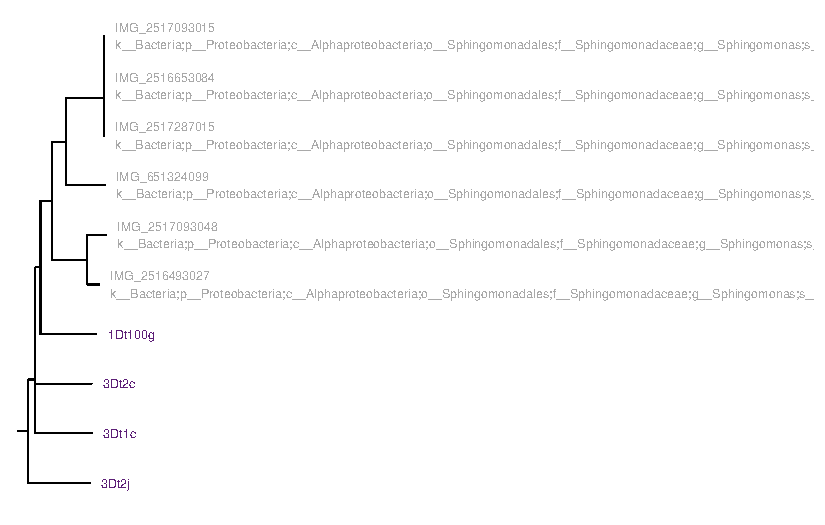
\includegraphics[width=0.9\linewidth,height=\textheight,keepaspectratio]{checkm_files/figure-pdf/fig-mtreeqasphingo-1.pdf}

}

\caption{\label{fig-mtreeqasphingo}Phylogram for 4 samples known to be
of the genus \emph{Sphingomonas}. Generated by checkm tree\_qa on the
30th of December 2024.}

\end{figure}%

\subsubsection{\texorpdfstring{\emph{Microbacterium}
samples}{Microbacterium samples}}

\begin{figure}

\centering{

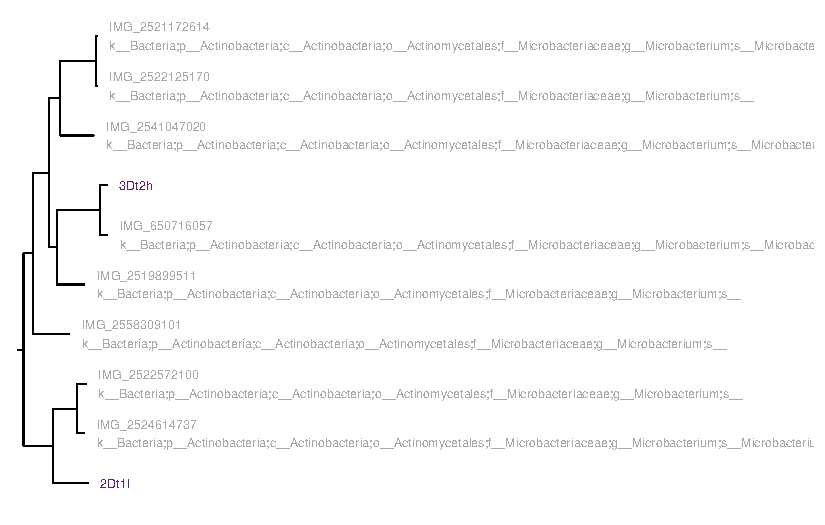
\includegraphics[width=0.9\linewidth,height=\textheight,keepaspectratio]{checkm_files/figure-pdf/fig-mtreeqamicro-1.pdf}

}

\caption{\label{fig-mtreeqamicro}Phylogram for 2 samples known to be of
the genus \emph{Microbacterium}. Generated by checkm tree\_qa on the
30th of December 2024.}

\end{figure}%

\subsubsection{\texorpdfstring{\emph{Brachybacterium / Dermabacter}
sample}{Brachybacterium / Dermabacter sample}}

\begin{figure}

\centering{

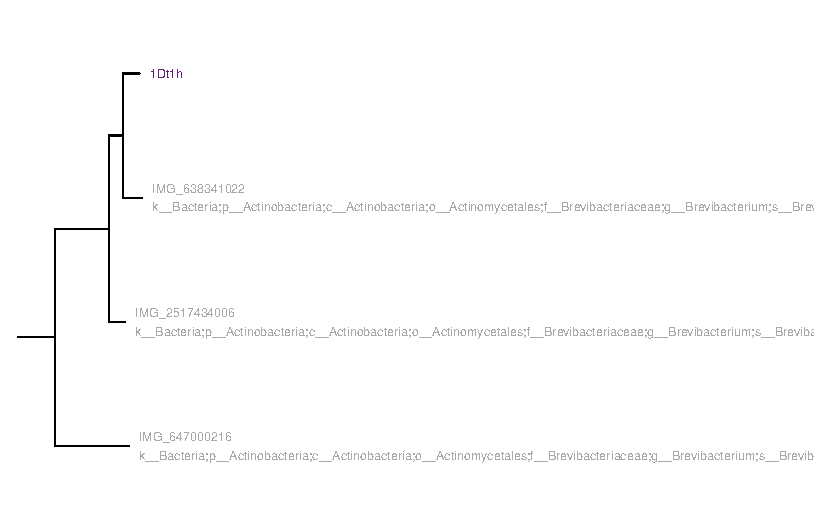
\includegraphics[width=0.9\linewidth,height=\textheight,keepaspectratio]{checkm_files/figure-pdf/fig-mtreeqabrach-1.pdf}

}

\caption{\label{fig-mtreeqabrach}Phylogram for 1 sample known to be of
the genus \emph{Brachybacterium}. Generated by checkm tree\_qa on the
30th of December 2024.}

\end{figure}%

\subsubsection{\texorpdfstring{\emph{Brevibacterium}
sample}{Brevibacterium sample}}

\begin{figure}

\centering{

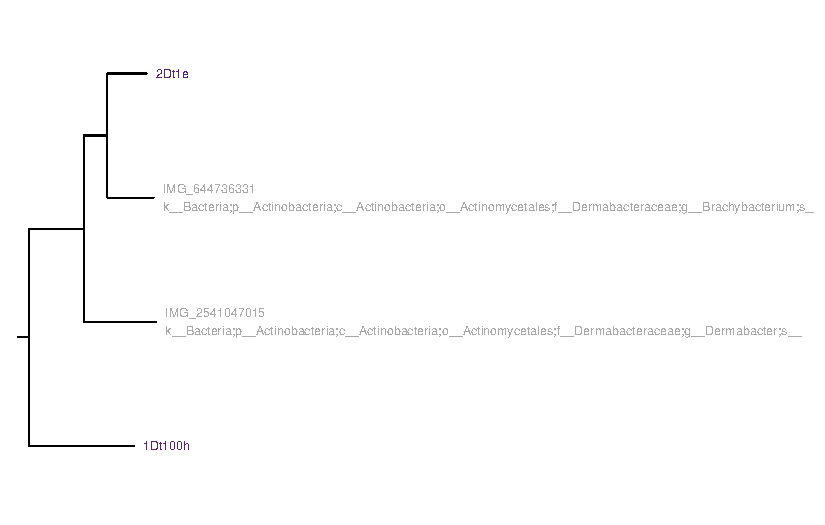
\includegraphics[width=0.9\linewidth,height=\textheight,keepaspectratio]{checkm_files/figure-pdf/fig-mtreeqabrev-1.pdf}

}

\caption{\label{fig-mtreeqabrev}Phylogram for 1 sample known to be of
the genus \emph{Brevibacterium}. Generated by checkm tree\_qa on the
30th of December 2024.}

\end{figure}%

\subsubsection{\texorpdfstring{\emph{Pantoea} sample}{Pantoea sample}}

\begin{figure}

\centering{

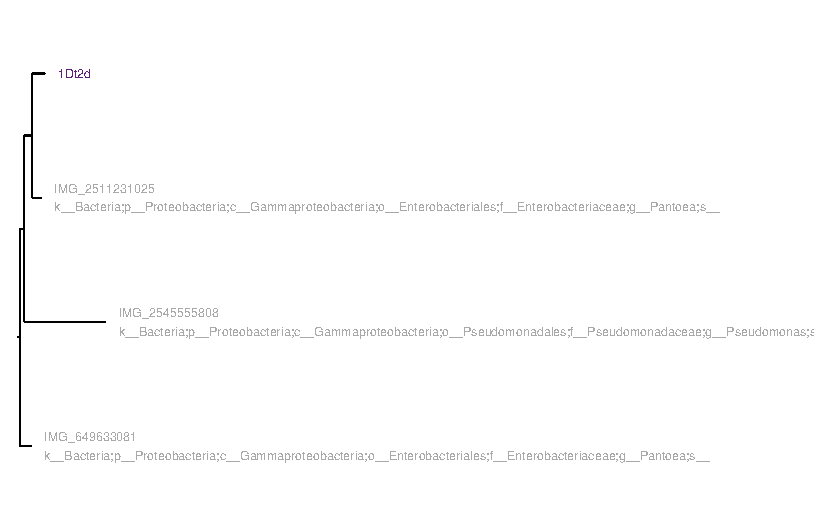
\includegraphics[width=0.9\linewidth,height=\textheight,keepaspectratio]{checkm_files/figure-pdf/fig-mtreeqapant-1.pdf}

}

\caption{\label{fig-mtreeqapant}Phylogram for 1 sample of disputed
genus. Generated by checkm tree\_qa on the 30th of December 2024.}

\end{figure}%

Outputs 3 and 4 produce the same tree files, with some minor differences
in labeling, so i have only outputted the results from the one that
returns the full taxonomic ID of each sample in the tip label. The trees
look to be trustworthy, confirming previous taxonomic assignments i have
run. It should be noted these use the IMG database, not the NCBI
database, this looks to be a smaller database as many of our samples are
outgroups on the trees with no direct sister samples, this can be seen
most for Figure 2, with all 4 samples in the outgroup. This analysis
does confirm again that sample 1Dt2d identified first as
``\emph{Enterobacter cancerogenus}'' is in fact a species of the genus
``\emph{Pantoea}''. As mentioned above i am yet to figure out if i can
do anything with the output from
\href{https://github.com/tobiasnunn/tnunn_research/blob/ddd084a8ec1dd159242afa64ee549ce588bf5ec7/02_middle-analysis_outputs/CheckM/checkmtreeqa/checkmtreeqa_msa.txt}{option
5}, so i will discuss with Aaron when term time begins again. Many of
the samples cannot be given a species name by this analysis, for
example, all of the samples in the genus \emph{Sphingomonas} are closest
to each other, so it is hard to discern if they are of different
species.

\section{Conclusion}\label{conclusion-1}

Output 2, and to a lesser extent 1, present interesting data, it is not
as useful as the data produced by the main analysis, but i think it was
worth doing. It is possible i am not fully apreciating all of the
outputs of this. Only very few of the samples get a taxonomy to the
species level, however, it does confirm that sample 1Dt2d, marked
``\emph{Enterobacter cancerogenus}'' by early taxonomic analysis
actually belongs to the genus \emph{Pantoea.} Confirming the analysis
done all the way back in the technical spike for gtdbtk de novo
\hyperref[conclusion]{Conclusion}. This is mirrored in the outputs of
the phylogenetic trees, which are good, but i doubt are a suitable
replacement for the ones output by gtdbtk, which i will get onto at some
point in the future. I have mentioned 5 several times, so i will just
say that i might come back to look at it later. I learned some new
things vis a vis new functions to tabulate like changing text size and
pruning/collapsing trees in R, so i am less reliant on dendroscope, and
have less tree files floating around. Overall, i think this has been a
useful thing to do, even if the outputs are not as important or useful
as what i have done or am about to do, even just for the experience
alone, but who knows, maybe there is something in this data that will be
useful to someone reading this.

\subsection{Scripts}\label{scripts-1}

\begin{itemize}
\item
  \href{https://github.com/tobiasnunn/tnunn_research/blob/3d90f340592d7081d3c6e172cbc786c8b85f368f/00_scripts/checkMtreeqa.sh}{checkMtreeqa.sh}
\item
  \href{https://github.com/tobiasnunn/tnunn_research/blob/20d1f52225ae83ba449e471cd260ce62f92c4ed9/00_scripts/CheckMtreeqa.R}{CheckMtreeqa.R}
\end{itemize}

\bookmarksetup{startatroot}

\chapter{CheckM2}\label{checkm2}

\section{Introduction}\label{introduction-5}

CheckM2 is a basic secondary analysis to test the quality of the samples
provided with a score for completeness and contamination (Chklovski et
al. 2023).

\section{Methods}\label{methods-3}

\subsection{CheckM2: slurm job}\label{checkm2-slurm-job}

I used the script
\href{https://github.com/tobiasnunn/tnunn_research/blob/main/Research_Experience_Module/00_scripts/Slurmscripts/run_checkm2TN.sh}{run\_checkm2TN.sh}
to run CheckM2 on all 10 fasta files at once.

\subsection{CheckM2: R table
generation}\label{checkm2-r-table-generation}

The CheckM2 job produced a
\href{https://github.com/tobiasnunn/tnunn_research/tree/main/Research_Experience_Module/02_middle-analysis_outputs/CheckM2_20241228}{set
of files}:

\begin{longtable}[]{@{}l@{}}

\caption{\label{tbl-files}CheckM2 output files}

\tabularnewline

\toprule\noalign{}
Filename \\
\midrule\noalign{}
\endhead
\bottomrule\noalign{}
\endlastfoot
checkM2comparison.xlsx \\
cumcomb.csv \\
diamond\_output/DIAMOND\_RESULTS.tsv \\
diamondko.csv \\
eggnogko.csv \\
protein\_files/flye\_asm\_1Dt100g\_part2.faa \\
protein\_files/flye\_asm\_1Dt100h\_part2.faa \\
protein\_files/flye\_asm\_1Dt1h\_part2.faa \\
protein\_files/flye\_asm\_1Dt2d\_part2.faa \\
protein\_files/flye\_asm\_2Dt1e\_part2.faa \\
protein\_files/flye\_asm\_2Dt1l\_part2.faa \\
protein\_files/flye\_asm\_3Dt1c\_part2.faa \\
protein\_files/flye\_asm\_3Dt2c\_part2.faa \\
protein\_files/flye\_asm\_3Dt2h\_part2.faa \\
protein\_files/flye\_asm\_3Dt2j\_part2.faa \\
quality\_report.tsv \\
uniquecomp.csv \\

\end{longtable}

The file I needed was \texttt{quality\_report.tsv}, which gives info on
each sample:

\begin{itemize}
\item
  Completeness
\item
  Contamination
\item
  Completeness Model Used
\item
  Translation Table Used
\end{itemize}

I created an R script
\href{https://github.com/tobiasnunn/tnunn_research/blob/main/Research_Experience_Module/00_scripts/Rscripts/CheckM2tablegenerator.R}{CheckM2tablegenerator.R.}
This produced Table~\ref{tbl-m2}

\begin{longtable}[]{@{}
  >{\raggedright\arraybackslash}p{(\linewidth - 22\tabcolsep) * \real{0.3333}}
  >{\raggedright\arraybackslash}p{(\linewidth - 22\tabcolsep) * \real{0.2828}}
  >{\raggedleft\arraybackslash}p{(\linewidth - 22\tabcolsep) * \real{0.0505}}
  >{\raggedleft\arraybackslash}p{(\linewidth - 22\tabcolsep) * \real{0.0404}}
  >{\raggedleft\arraybackslash}p{(\linewidth - 22\tabcolsep) * \real{0.0404}}
  >{\raggedleft\arraybackslash}p{(\linewidth - 22\tabcolsep) * \real{0.0303}}
  >{\raggedleft\arraybackslash}p{(\linewidth - 22\tabcolsep) * \real{0.0303}}
  >{\raggedleft\arraybackslash}p{(\linewidth - 22\tabcolsep) * \real{0.0404}}
  >{\raggedleft\arraybackslash}p{(\linewidth - 22\tabcolsep) * \real{0.0303}}
  >{\raggedleft\arraybackslash}p{(\linewidth - 22\tabcolsep) * \real{0.0404}}
  >{\raggedleft\arraybackslash}p{(\linewidth - 22\tabcolsep) * \real{0.0404}}
  >{\raggedleft\arraybackslash}p{(\linewidth - 22\tabcolsep) * \real{0.0404}}@{}}

\caption{\label{tbl-diamond}First five rows of DIAMOND\_RESULTS.tsv
file}

\tabularnewline

\toprule\noalign{}
\begin{minipage}[b]{\linewidth}\raggedright
V1
\end{minipage} & \begin{minipage}[b]{\linewidth}\raggedright
V2
\end{minipage} & \begin{minipage}[b]{\linewidth}\raggedleft
V3
\end{minipage} & \begin{minipage}[b]{\linewidth}\raggedleft
V4
\end{minipage} & \begin{minipage}[b]{\linewidth}\raggedleft
V5
\end{minipage} & \begin{minipage}[b]{\linewidth}\raggedleft
V6
\end{minipage} & \begin{minipage}[b]{\linewidth}\raggedleft
V7
\end{minipage} & \begin{minipage}[b]{\linewidth}\raggedleft
V8
\end{minipage} & \begin{minipage}[b]{\linewidth}\raggedleft
V9
\end{minipage} & \begin{minipage}[b]{\linewidth}\raggedleft
V10
\end{minipage} & \begin{minipage}[b]{\linewidth}\raggedleft
V11
\end{minipage} & \begin{minipage}[b]{\linewidth}\raggedleft
V12
\end{minipage} \\
\midrule\noalign{}
\endhead
\bottomrule\noalign{}
\endlastfoot
flye\_asm\_1Dt1h\_part2Ωcontig\_2\_1 &
UniRef100\_E8NCL3\textasciitilde K07154 & 49.7 & 396 & 196 & 2 & 18 &
411 & 17 & 411 & 0 & 354 \\
flye\_asm\_1Dt1h\_part2Ωcontig\_3\_3 &
UniRef100\_A0A142NN80\textasciitilde K01866 & 91.8 & 428 & 35 & 0 & 1 &
428 & 1 & 428 & 0 & 767 \\
flye\_asm\_1Dt1h\_part2Ωcontig\_3\_7 &
UniRef100\_A0A0M4DMT0\textasciitilde K03088 & 44.0 & 407 & 224 & 2 & 2 &
404 & 8 & 414 & 0 & 313 \\
flye\_asm\_1Dt1h\_part2Ωcontig\_3\_9 &
UniRef100\_A0A142NQF8\textasciitilde K01755 & 93.0 & 473 & 33 & 0 & 1 &
473 & 1 & 473 & 0 & 857 \\
flye\_asm\_1Dt1h\_part2Ωcontig\_3\_10 &
UniRef100\_A0A142NNT5\textasciitilde K03402 & 93.5 & 168 & 11 & 0 & 8 &
175 & 6 & 173 & 0 & 282 \\

\end{longtable}

\subsection{Results}\label{results-2}

\begin{table}

\caption{\label{tbl-m2}Quality analysis from CheckM2 based on samples
taken from the skin microbiome of \emph{Dendrobates tinctorius}}

\centering{

\fontsize{12.0pt}{14.4pt}\selectfont
\begin{tabular*}{\linewidth}{@{\extracolsep{\fill}}lrr>{\raggedright\arraybackslash}p{\dimexpr 187.50pt -2\tabcolsep-1.5\arrayrulewidth}rl}
\toprule
Accession & Completeness & Contamination & Completeness model used & Translation table used & Additional notes \\ 
\midrule\addlinespace[2.5pt]
1Dt1h & {\cellcolor[HTML]{08306B}{\textcolor[HTML]{FFFFFF}{100.00}}} & {\cellcolor[HTML]{FEE9D3}{\textcolor[HTML]{000000}{0.31}}} & Neural Network (Specific Model) & 11 & None \\ 
1Dt2d & {\cellcolor[HTML]{08306B}{\textcolor[HTML]{FFFFFF}{100.00}}} & {\cellcolor[HTML]{FEC590}{\textcolor[HTML]{000000}{0.87}}} & Neural Network (Specific Model) & 11 & None \\ 
2Dt1l & {\cellcolor[HTML]{08306B}{\textcolor[HTML]{FFFFFF}{100.00}}} & {\cellcolor[HTML]{FEEAD6}{\textcolor[HTML]{000000}{0.27}}} & Neural Network (Specific Model) & 11 & None \\ 
3Dt2c & {\cellcolor[HTML]{08326D}{\textcolor[HTML]{FFFFFF}{99.94}}} & {\cellcolor[HTML]{FEE5CC}{\textcolor[HTML]{000000}{0.39}}} & Neural Network (Specific Model) & 11 & None \\ 
3Dt2j & {\cellcolor[HTML]{083573}{\textcolor[HTML]{FFFFFF}{99.80}}} & {\cellcolor[HTML]{FFF5EB}{\textcolor[HTML]{000000}{0.00}}} & Neural Network (Specific Model) & 11 & None \\ 
1Dt100h & {\cellcolor[HTML]{09478D}{\textcolor[HTML]{FFFFFF}{99.12}}} & {\cellcolor[HTML]{FFF5EB}{\textcolor[HTML]{000000}{0.00}}} & Gradient Boost (General Model) & 11 & None \\ 
3Dt1c & {\cellcolor[HTML]{135BA4}{\textcolor[HTML]{FFFFFF}{98.34}}} & {\cellcolor[HTML]{FEC692}{\textcolor[HTML]{000000}{0.86}}} & Neural Network (Specific Model) & 11 & None \\ 
3Dt2h & {\cellcolor[HTML]{808080}{\textcolor[HTML]{FFFFFF}{86.04}}} & {\cellcolor[HTML]{FFF1E3}{\textcolor[HTML]{000000}{0.10}}} & Neural Network (Specific Model) & 11 & None \\ 
1Dt100g & {\cellcolor[HTML]{808080}{\textcolor[HTML]{FFFFFF}{78.42}}} & {\cellcolor[HTML]{FEE8D1}{\textcolor[HTML]{000000}{0.33}}} & Neural Network (Specific Model) & 11 & None \\ 
2Dt1e & {\cellcolor[HTML]{808080}{\textcolor[HTML]{FFFFFF}{48.29}}} & {\cellcolor[HTML]{FFF2E5}{\textcolor[HTML]{000000}{0.08}}} & Neural Network (Specific Model) & 11 & None \\ 
\bottomrule
\end{tabular*}
\begin{minipage}{\linewidth}
Source: CheckM2 predict performed on 2024-12-28\\
\end{minipage}

}

\end{table}%

This is the table of CheckM2 analysis, there are many differences in
which fields are produced, also, there appears to be differences in the
values themselves for Completeness and Contamination, perhaps part of
the comparitive analysis, done in the conclusion should be the date at
which both were at, as older versions will probably have less accurate
values, and this may cause the difference as genomics is a fast evolving
field. A noteable difference is that CheckM used an internal diamond
database, whereas CheckM2 required me to download my own.

\subsection{Scripts}\label{scripts-2}

\begin{itemize}
\item
  \href{https://github.com/tobiasnunn/tnunn_research/blob/main/Research_Experience_Module/00_scripts/Slurmscripts/run_checkm2TN.sh}{run\_checkm2TN.sh}
\item
  \href{https://github.com/tobiasnunn/tnunn_research/blob/main/Research_Experience_Module/00_scripts/Rscripts/CheckM2tablegenerator.R}{CheckM2tablegenerator.R.}
\end{itemize}

\subsection{Comparison of CheckM and
CheckM2}\label{comparison-of-checkm-and-checkm2}

\begin{table}

\caption{\label{tbl-mm2}Comparison of quality metrics for the same fasta
files between CheckM/1.1.3 and CheckM2/0.1.3}

\centering{

\fontsize{12.0pt}{14.4pt}\selectfont
\begin{tabular*}{\linewidth}{@{\extracolsep{\fill}}lrrrr}
\toprule
 & \multicolumn{2}{c}{CheckM/1.1.3} & \multicolumn{2}{c}{CheckM2/0.1.3} \\ 
\cmidrule(lr){2-3} \cmidrule(lr){4-5}
Accession & Completeness & Contamination & Completeness & Contamination \\ 
\midrule\addlinespace[2.5pt]
1Dt100g & {\cellcolor[HTML]{808080}{\textcolor[HTML]{FFFFFF}{76.77}}} & {\cellcolor[HTML]{FFF5EB}{\textcolor[HTML]{000000}{0.00}}} & {\cellcolor[HTML]{808080}{\textcolor[HTML]{FFFFFF}{78.42}}} & {\cellcolor[HTML]{FEE8D1}{\textcolor[HTML]{000000}{0.33}}} \\ 
1Dt100h & {\cellcolor[HTML]{084E98}{\textcolor[HTML]{FFFFFF}{98.84}}} & {\cellcolor[HTML]{FFEDDC}{\textcolor[HTML]{000000}{0.19}}} & {\cellcolor[HTML]{09478D}{\textcolor[HTML]{FFFFFF}{99.12}}} & {\cellcolor[HTML]{FFF5EB}{\textcolor[HTML]{000000}{0.00}}} \\ 
1Dt1h & {\cellcolor[HTML]{08306B}{\textcolor[HTML]{FFFFFF}{100.00}}} & {\cellcolor[HTML]{FFF5EB}{\textcolor[HTML]{000000}{0.00}}} & {\cellcolor[HTML]{08306B}{\textcolor[HTML]{FFFFFF}{100.00}}} & {\cellcolor[HTML]{FEE9D3}{\textcolor[HTML]{000000}{0.31}}} \\ 
1Dt2d & {\cellcolor[HTML]{08306B}{\textcolor[HTML]{FFFFFF}{100.00}}} & {\cellcolor[HTML]{FEC38D}{\textcolor[HTML]{000000}{0.90}}} & {\cellcolor[HTML]{08306B}{\textcolor[HTML]{FFFFFF}{100.00}}} & {\cellcolor[HTML]{FEC590}{\textcolor[HTML]{000000}{0.87}}} \\ 
2Dt1e & {\cellcolor[HTML]{808080}{\textcolor[HTML]{FFFFFF}{44.74}}} & {\cellcolor[HTML]{FFF5EB}{\textcolor[HTML]{000000}{0.00}}} & {\cellcolor[HTML]{808080}{\textcolor[HTML]{FFFFFF}{48.29}}} & {\cellcolor[HTML]{FFF2E5}{\textcolor[HTML]{000000}{0.08}}} \\ 
2Dt1l & {\cellcolor[HTML]{084F99}{\textcolor[HTML]{FFFFFF}{98.82}}} & {\cellcolor[HTML]{D04502}{\textcolor[HTML]{FFFFFF}{2.32}}} & {\cellcolor[HTML]{08306B}{\textcolor[HTML]{FFFFFF}{100.00}}} & {\cellcolor[HTML]{FEEAD6}{\textcolor[HTML]{000000}{0.27}}} \\ 
3Dt1c & {\cellcolor[HTML]{2A78B9}{\textcolor[HTML]{FFFFFF}{97.23}}} & {\cellcolor[HTML]{FDA862}{\textcolor[HTML]{000000}{1.19}}} & {\cellcolor[HTML]{135BA4}{\textcolor[HTML]{FFFFFF}{98.34}}} & {\cellcolor[HTML]{FEC692}{\textcolor[HTML]{000000}{0.86}}} \\ 
3Dt2c & {\cellcolor[HTML]{549DCC}{\textcolor[HTML]{FFFFFF}{95.75}}} & {\cellcolor[HTML]{FEC793}{\textcolor[HTML]{000000}{0.85}}} & {\cellcolor[HTML]{08326D}{\textcolor[HTML]{FFFFFF}{99.94}}} & {\cellcolor[HTML]{FEE5CC}{\textcolor[HTML]{000000}{0.39}}} \\ 
3Dt2h & {\cellcolor[HTML]{808080}{\textcolor[HTML]{FFFFFF}{87.98}}} & {\cellcolor[HTML]{FEDEBF}{\textcolor[HTML]{000000}{0.51}}} & {\cellcolor[HTML]{808080}{\textcolor[HTML]{FFFFFF}{86.04}}} & {\cellcolor[HTML]{FFF1E3}{\textcolor[HTML]{000000}{0.10}}} \\ 
3Dt2j & {\cellcolor[HTML]{4493C7}{\textcolor[HTML]{FFFFFF}{96.19}}} & {\cellcolor[HTML]{FDA761}{\textcolor[HTML]{000000}{1.21}}} & {\cellcolor[HTML]{083573}{\textcolor[HTML]{FFFFFF}{99.80}}} & {\cellcolor[HTML]{FFF5EB}{\textcolor[HTML]{000000}{0.00}}} \\ 
\bottomrule
\end{tabular*}
\begin{minipage}{\linewidth}
Source:\\
CheckM lineage\_wf performed on 2024-12-25\\
CheckM2 predict performed on 2024-12-28\\
\end{minipage}

}

\end{table}%

\section{CheckM2
DIAMOND\_RESULTS.tsv}\label{checkm2-diamond_results.tsv}

\subsection{Introduction}\label{introduction-6}

I decided to take a look at the full outputs of CheckM2 to see if there
was anything interesting to analyse other than the Completeness and
Contamination, I found this file called
\href{https://github.com/tobiasnunn/tnunn_research/blob/main/Research_Experience_Module/02_middle-analysis_outputs/CheckM2_20241228/diamond_output/DIAMOND_RESULTS.tsv}{DIAMOND\_RESULTS.tsv}.
It has a bunch of weird stuff in it, I did however recognise the
existence of KO pathways in the second column, along with links to a
website that displays 3D images of proteins, so I decided to take a
closer look at this file.

\subsection{Methods}\label{methods-4}

The file did not output with column headers, I believe the ones found
\href{https://www.metagenomics.wiki/tools/blast/blastn-output-format-6}{here}
match up well, but the descriptions of some are vague, so I am not sure
what the significance of a few of the columns is. Due to the size of
DIAMOND\_RESULTS.tsv, I decided not to include it as a table or image in
this document. I created this
\href{https://github.com/tobiasnunn/tnunn_research/blob/main/Research_Experience_Module/00_scripts/Rscripts/CheckM2diamondanalysis.R}{R
script} to import the data to a table and do an analysis of the
important looking fields. This was quite a difficult task that made this
little project stretch over 2 days. The main output I wanted from this
was a comparison between the KO pathways outputted from this and those
outputted by Eggnog-mapper. Eggnog-mapper still is not working on Hawk
so maybe we could get the KO pathways for the heatmaps through CheckM2
instead. I did this analysis at two levels, a comparison of which unique
KOs each system recognised, and the ``cumulative'' or total differences.

I figured if I am going to make decisions based on if two methods are
different, I should compare them statistically instead of eyeballing it.
It is simple enough, tests, graphs, that sort of stuff. This lead me to
do many things in R, but only some of the analyses I did were valid. I
started off testing which KO values against which accessions in each
file, excluding repetitions. However, I then realised that this
methodology did not give a full picture of the results, so I decided to
work on trying to identify when duplicates occured and add them to the
dataset. After much trial and error to get right, I created
\href{https://github.com/tobiasnunn/tnunn_research/blob/main/Research_Experience_Module/00_scripts/Rscripts/CheckM2diamondanalysis.R}{this
file}. I included all the dead-ends as comments at the end for
posterity. I finally decided to use the shared KO values divided by the
total for each accession and method to create my values showing the
differences between DIAMOND and eggNog-mapper. I then decided to run a
statistical analysis to see if the differences observed between groups
was significant.

\subsection{Results}\label{results-3}

\begin{figure}

\centering{

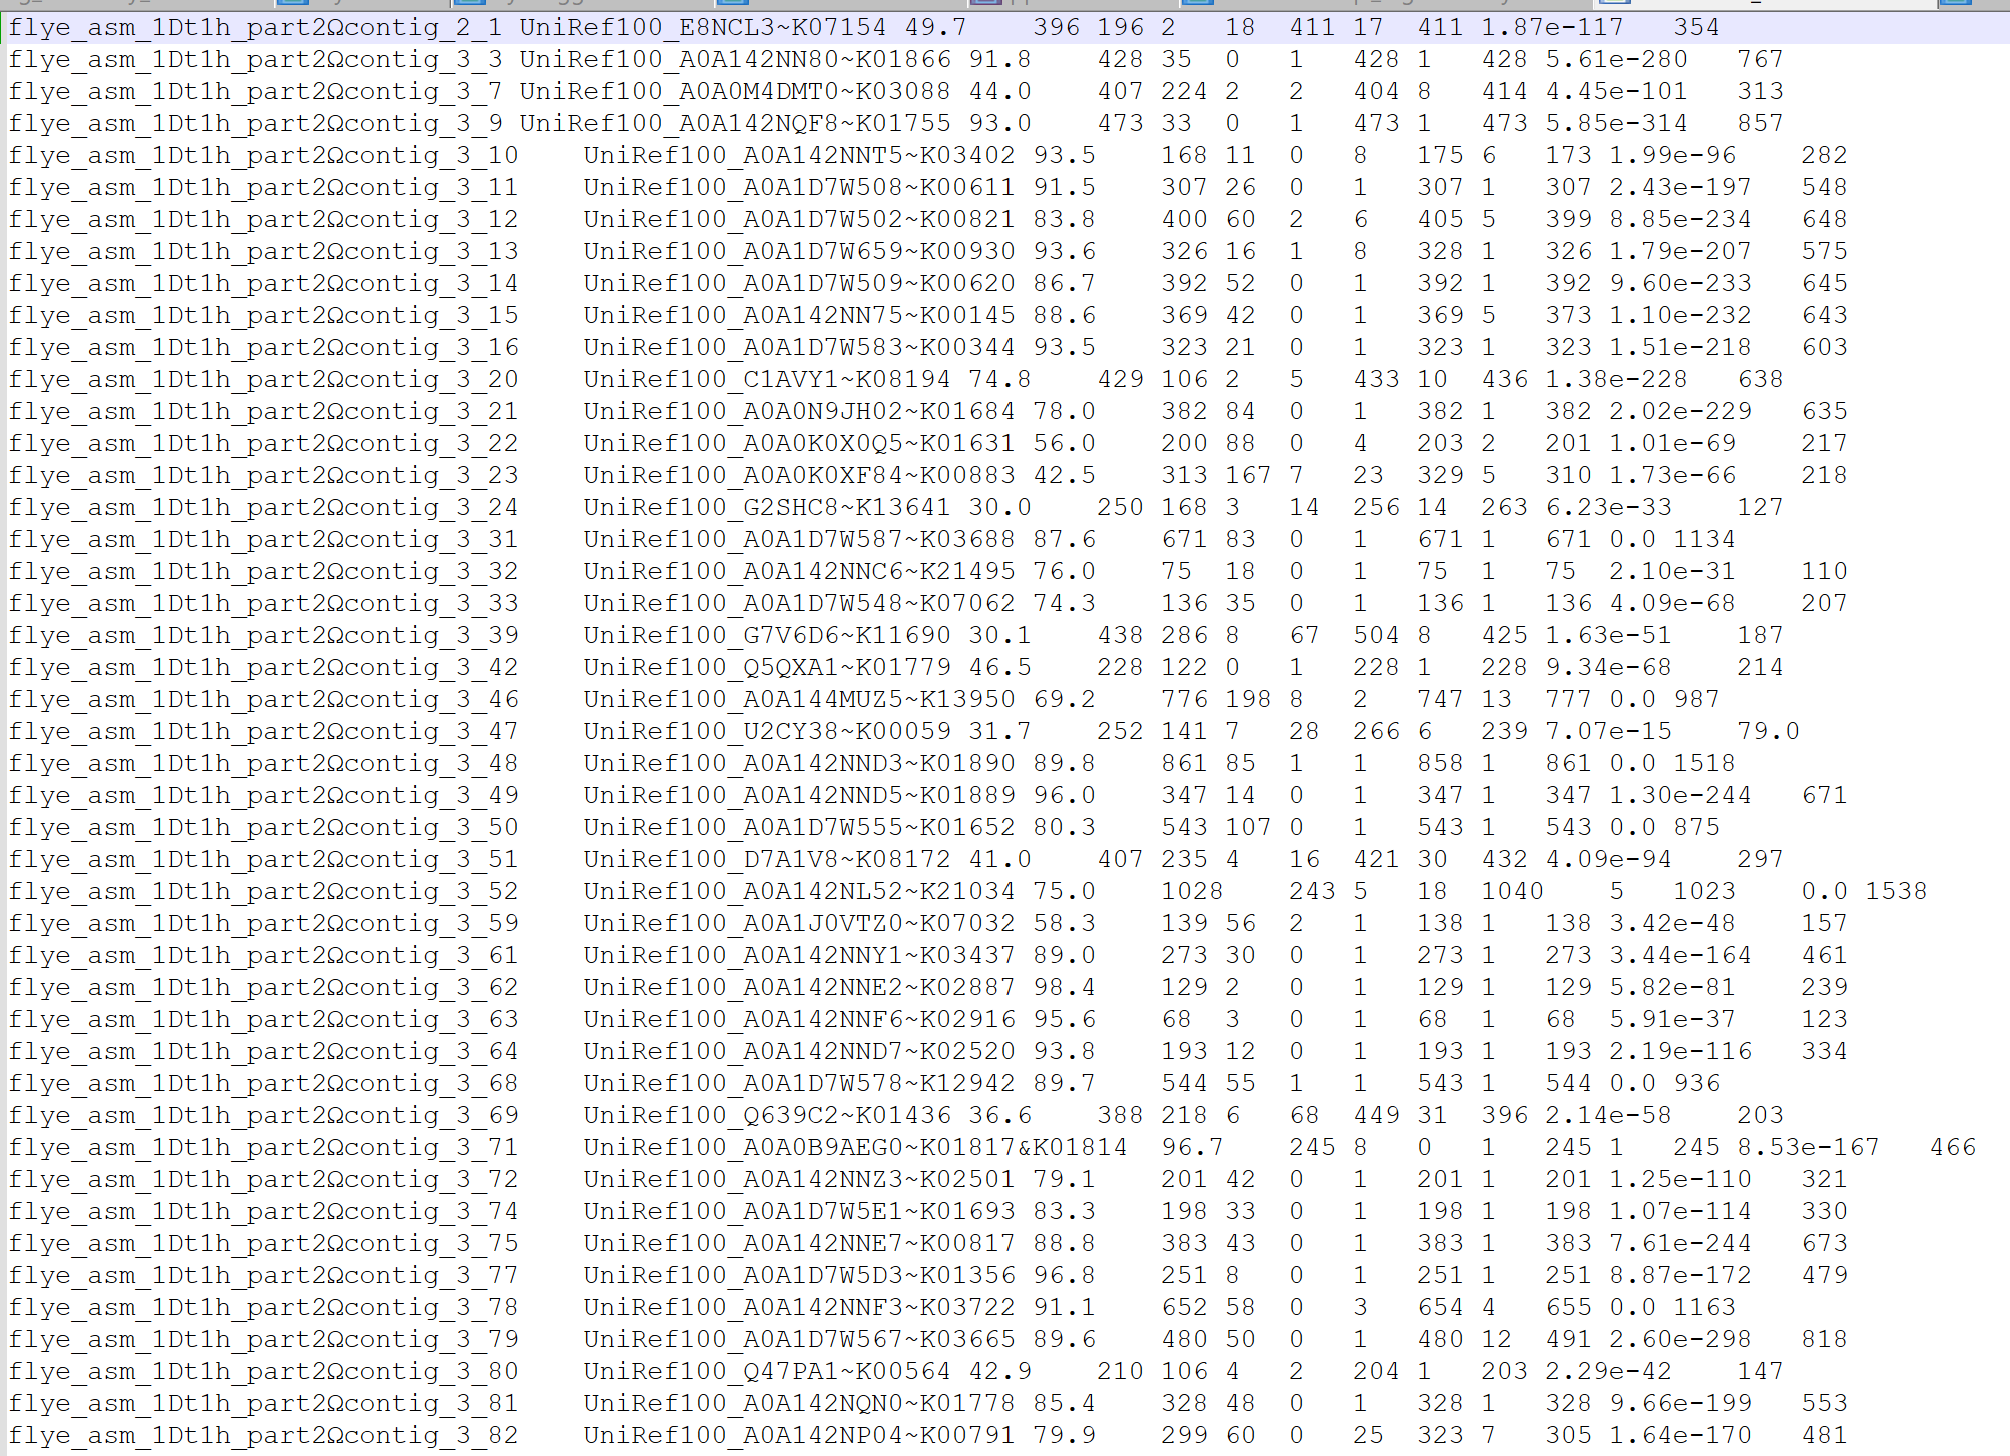
\includegraphics[width=6.7in,height=\textheight,keepaspectratio]{img/DIAMOND_RESULTS.tsv.png}

}

\caption{\label{fig-diamond}The original file is very large, so I cannot
include it in the document, there is a line for each gene in all 10
samples. Here is a screenshot of it in Notepad ++}

\end{figure}%

\begin{table}

\caption{\label{tbl-2other}Unique KO pathway analysis from CheckM2 based
on samples taken from the skin microbiome of \emph{Dendrobates
tinctorius}}

\centering{

\fontsize{12.0pt}{14.4pt}\selectfont
\begin{tabular*}{\linewidth}{@{\extracolsep{\fill}}lrrrrr}
\toprule
Accession & Total unique KOs & KO \# in DIAMOND file & KO \# from eggNog-mapper files & \% diff DIAMOND - eggNog & \% diff eggNog - DIAMOND \\ 
\midrule\addlinespace[2.5pt]
1Dt100g & 1160 & 1096 & 1034 & 0.9448276 & 0.8913793 \\ 
1Dt100h & 1179 & 1055 & 1107 & 0.8948261 & 0.9389313 \\ 
1Dt1h & 1627 & 1505 & 1466 & 0.9250154 & 0.9010449 \\ 
1Dt2d & 2856 & 2631 & 2702 & 0.9212185 & 0.9460784 \\ 
2Dt1e & 966 & 828 & 854 & 0.8571429 & 0.8840580 \\ 
2Dt1l & 1641 & 1471 & 1467 & 0.8964046 & 0.8939671 \\ 
3Dt1c & 1641 & 1572 & 1438 & 0.9579525 & 0.8762949 \\ 
3Dt2c & 1654 & 1582 & 1447 & 0.9564692 & 0.8748489 \\ 
3Dt2h & 1411 & 1254 & 1280 & 0.8887314 & 0.9071580 \\ 
3Dt2j & 1475 & 1428 & 1302 & 0.9681356 & 0.8827119 \\ 
\bottomrule
\end{tabular*}
\begin{minipage}{\linewidth}
Source: DIAMOND\_RESULTS.tsv produced by CheckM2 predict performed on 2024-12-28\\
\end{minipage}

}

\end{table}%

\begin{table}

\caption{\label{tbl-2otherother}KO pathway Total Frequency analysis from
CheckM2 based on samples taken from the skin microbiome of
\emph{Dendrobates tinctorius}}

\centering{

\fontsize{12.0pt}{14.4pt}\selectfont
\begin{tabular*}{\linewidth}{@{\extracolsep{\fill}}llrllr}
\toprule
Accession & EggNog-mapper most-frequent KO pathways & Ocurrance number in genome & accession.d & DIAMOND most-frequent KO pathways & Ocurrance number in genome \\ 
\midrule\addlinespace[2.5pt]
1Dt100g & K00799 & 8 & 1Dt100g & K00249 & 11 \\ 
1Dt100g & K02014 & 6 & 1Dt100g & K00059 & 8 \\ 
1Dt100g & K00626 & 4 & 1Dt100g & K02014 & 8 \\ 
1Dt100g & K00666 & 4 & 1Dt100g & K00799 & 7 \\ 
1Dt100g & K11177 & 4 & 1Dt100g & K01069 & 4 \\ 
1Dt100h & K02015 & 8 & 1Dt100h & K02015 & 8 \\ 
1Dt100h & K01990 & 7 & 1Dt100h & K01990 & 6 \\ 
1Dt100h & K02013 & 6 & 1Dt100h & K02013 & 6 \\ 
1Dt100h & K02016 & 6 & 1Dt100h & K02016 & 6 \\ 
1Dt100h & K02031 & 6 & 1Dt100h & K02031 & 5 \\ 
1Dt1h & K02016 & 18 & 1Dt1h & K00059 & 21 \\ 
1Dt1h & K00059 & 13 & 1Dt1h & K02016 & 18 \\ 
1Dt1h & K01990 & 12 & 1Dt1h & K02031 & 11 \\ 
1Dt1h & K01992 & 11 & 1Dt1h & K02032 & 11 \\ 
1Dt1h & K02031 & 11 & 1Dt1h & K07749 & 11 \\ 
1Dt2d & K02029 & 28 & 1Dt2d & K18900 & 21 \\ 
1Dt2d & K03406 & 21 & 1Dt2d & K07495 & 16 \\ 
1Dt2d & K02031 & 17 & 1Dt2d & K00059 & 15 \\ 
1Dt2d & K02028 & 14 & 1Dt2d & K02029 & 15 \\ 
1Dt2d & K02032 & 14 & 1Dt2d & K02529 & 15 \\ 
2Dt1e & K02026 & 20 & 2Dt1e & K02026 & 19 \\ 
2Dt1e & K02027 & 18 & 2Dt1e & K02025 & 18 \\ 
2Dt1e & K02025 & 15 & 2Dt1e & K02027 & 17 \\ 
2Dt1e & K06147 & 9 & 2Dt1e & K02529 & 12 \\ 
2Dt1e & K02529 & 8 & 2Dt1e & K06147 & 9 \\ 
2Dt1l & K02034 & 30 & 2Dt1l & K02529 & 30 \\ 
2Dt1l & K02035 & 28 & 2Dt1l & K02031 & 27 \\ 
2Dt1l & K02031 & 26 & 2Dt1l & K02035 & 25 \\ 
2Dt1l & K02033 & 26 & 2Dt1l & K02032 & 24 \\ 
2Dt1l & K02025 & 22 & 2Dt1l & K02033 & 24 \\ 
3Dt1c & K02014 & 24 & 3Dt1c & K02014 & 40 \\ 
3Dt1c & K03406 & 14 & 3Dt1c & K03406 & 16 \\ 
3Dt1c & K14266 & 11 & 3Dt1c & K14266 & 14 \\ 
3Dt1c & K02529 & 7 & 3Dt1c & K02529 & 8 \\ 
3Dt1c & K03088 & 7 & 3Dt1c & K05349 & 8 \\ 
3Dt2c & K02014 & 23 & 3Dt2c & K02014 & 35 \\ 
3Dt2c & K03406 & 17 & 3Dt2c & K07497 & 18 \\ 
3Dt2c & K14266 & 12 & 3Dt2c & K03406 & 17 \\ 
3Dt2c & K02483 & 7 & 3Dt2c & K14266 & 17 \\ 
3Dt2c & K03496 & 7 & 3Dt2c & K00059 & 8 \\ 
3Dt2h & K02529 & 14 & 3Dt2h & K02529 & 18 \\ 
3Dt2h & K02025 & 13 & 3Dt2h & K02025 & 11 \\ 
3Dt2h & K02026 & 13 & 3Dt2h & K02026 & 11 \\ 
3Dt2h & K02027 & 12 & 3Dt2h & K02027 & 11 \\ 
3Dt2h & K03088 & 9 & 3Dt2h & K03088 & 10 \\ 
3Dt2j & K02014 & 12 & 3Dt2j & K02014 & 21 \\ 
3Dt2j & K00626 & 6 & 3Dt2j & K00249 & 9 \\ 
3Dt2j & K00799 & 6 & 3Dt2j & K00059 & 8 \\ 
3Dt2j & K07107 & 5 & 3Dt2j & K00799 & 8 \\ 
3Dt2j & K03088 & 4 & 3Dt2j & K01897 & 7 \\ 
\bottomrule
\end{tabular*}
\begin{minipage}{\linewidth}
Source: DIAMOND\_RESULTS.tsv produced by CheckM2 predict performed on 2024-12-28\\
\end{minipage}

}

\end{table}%

Table~\ref{tbl-2other} and Table~\ref{tbl-2otherother} represent my
analysis of the DIAMOND\_RESULTS.tsv file. I decided to do this by
comparing it to the outputs I got from eggNog-mapper when I ran it
earlier in the year. Table~\ref{tbl-2other} represents a comparison of
unique KO pathways. Often, the same KO pathway is found multiple times
in the same genome, this makes evolutionary sense but if CheckM2 is a
good alternative to eggNog-mapper, which does not work on hawk yet then
it must find similar KO pathways. Table~\ref{tbl-2other} would confirm
this as similarities between output files consistently stay above 85\%.
Table 8 represents a comparison of highest frequency, taken as the top 5
most frequent for each genome. Basically, what are each system finding
most often. Often, there will be similarities, with values only off by 2
or 3, however, occasionally the most common in DIAMOND will be absent
from the list for eggNog-mapper and vice-versa.

\subsection{Statistical analysis
results}\label{statistical-analysis-results}

\begin{table}

\caption{\label{tbl-finaldiamond}Shared KO values between two systems
represented as proportions of their totals based on samples taken from
the skin microbiome of \emph{Dendrobates tinctorius}}

\centering{

\fontsize{12.0pt}{14.4pt}\selectfont
\begin{tabular*}{\linewidth}{@{\extracolsep{\fill}}lrr}
\toprule
Accession & \% of shared KO values present in DIAMOND\_RESULTS.tsv & \% of shared KO values present in eggNog-mapper outputs \\ 
\midrule\addlinespace[2.5pt]
1Dt100g & 84.9\% & 92.0\% \\ 
1Dt100h & 91.5\% & 84.9\% \\ 
1Dt1h & 84.7\% & 87.3\% \\ 
1Dt2d & 88.4\% & 82.8\% \\ 
2Dt1e & 82.6\% & 82.1\% \\ 
2Dt1l & 83.4\% & 85.4\% \\ 
3Dt1c & 82.1\% & 94.1\% \\ 
3Dt2c & 80.7\% & 93.7\% \\ 
3Dt2h & 86.7\% & 83.4\% \\ 
3Dt2j & 84.1\% & 94.9\% \\ 
\bottomrule
\end{tabular*}
\begin{minipage}{\linewidth}
Source: DIAMOND\_RESULTS.tsv produced by CheckM2 predict performed on 2024-12-28 and the series of eggNog-mapper outputs I generated using eggNog-mapper v2 for the web 2024-08-28\\
\end{minipage}

}

\end{table}%

\begin{Shaded}
\begin{Highlighting}[]
\FunctionTok{shapiro.test}\NormalTok{(groupby}\SpecialCharTok{$}\NormalTok{DIAMOND\_per)}
\end{Highlighting}
\end{Shaded}

\begin{verbatim}

    Shapiro-Wilk normality test

data:  groupby$DIAMOND_per
W = 0.94467, p-value = 0.6061
\end{verbatim}

\begin{Shaded}
\begin{Highlighting}[]
\FunctionTok{shapiro.test}\NormalTok{(groupby}\SpecialCharTok{$}\NormalTok{eggNog\_per)}
\end{Highlighting}
\end{Shaded}

\begin{verbatim}

    Shapiro-Wilk normality test

data:  groupby$eggNog_per
W = 0.8645, p-value = 0.08619
\end{verbatim}

\begin{Shaded}
\begin{Highlighting}[]
\NormalTok{compttest }\OtherTok{\textless{}{-}} \FunctionTok{t.test}\NormalTok{(groupby}\SpecialCharTok{$}\NormalTok{DIAMOND\_per, groupby}\SpecialCharTok{$}\NormalTok{eggNog\_per)}
\NormalTok{compttest}
\end{Highlighting}
\end{Shaded}

\begin{verbatim}

    Welch Two Sample t-test

data:  groupby$DIAMOND_per and groupby$eggNog_per
t = -1.6563, df = 15.199, p-value = 0.1182
alternative hypothesis: true difference in means is not equal to 0
95 percent confidence interval:
 -0.07200294  0.00899259
sample estimates:
mean of x mean of y 
0.8490075 0.8805126 
\end{verbatim}

Table~\ref{tbl-finaldiamond} shows that the common KO values represent a
very large proportion of the total KO values for both methods and all
accessions, never dipping below 80\%. Shapiro testing showed that a
parametric test could be used for this. I decided on a Student's
t-test(t(15.199) = -1.6563, p = 0.1182). As the p value is larger than
0.05, we accept the null hypothesis that the groups are not
significantly different.

\bookmarksetup{startatroot}

\chapter{GTDB-TK Classify}\label{sec-classify}

\section{Introduction}\label{introduction-7}

In september, when I was still inexperienced, I ran GTDB-Tk on the 10
samples using the classify\_wf. At the time, that is the only way I
thought it could be used. I got a few trees output from this, but
because the trees were not monophyletic, so I discarded them as not
possible to be correct. However, there was another output that I did not
see or disregarded.

\section{Methods}\label{methods-5}

The script used was the same as in the de\_novo process.

\section{Results}\label{results-4}

\subsection{Table}\label{table}

The table was too large to include here, so here is a link to it in the
repo:
\href{https://github.com/tobiasnunn/tnunn_research/blob/6bfc481b8ebb4b2d3d0ec013bfe68a3662fb4ca4/Research_Experience_Module/02_middle-analysis_outputs/gtdbtk_stuff/classify_wf/gtdbtk.bac120.summary.tsv}{gtdbtk.bac120.summary.tsv}

\subsection{tree example}\label{tree-example}

\begin{figure}

\centering{

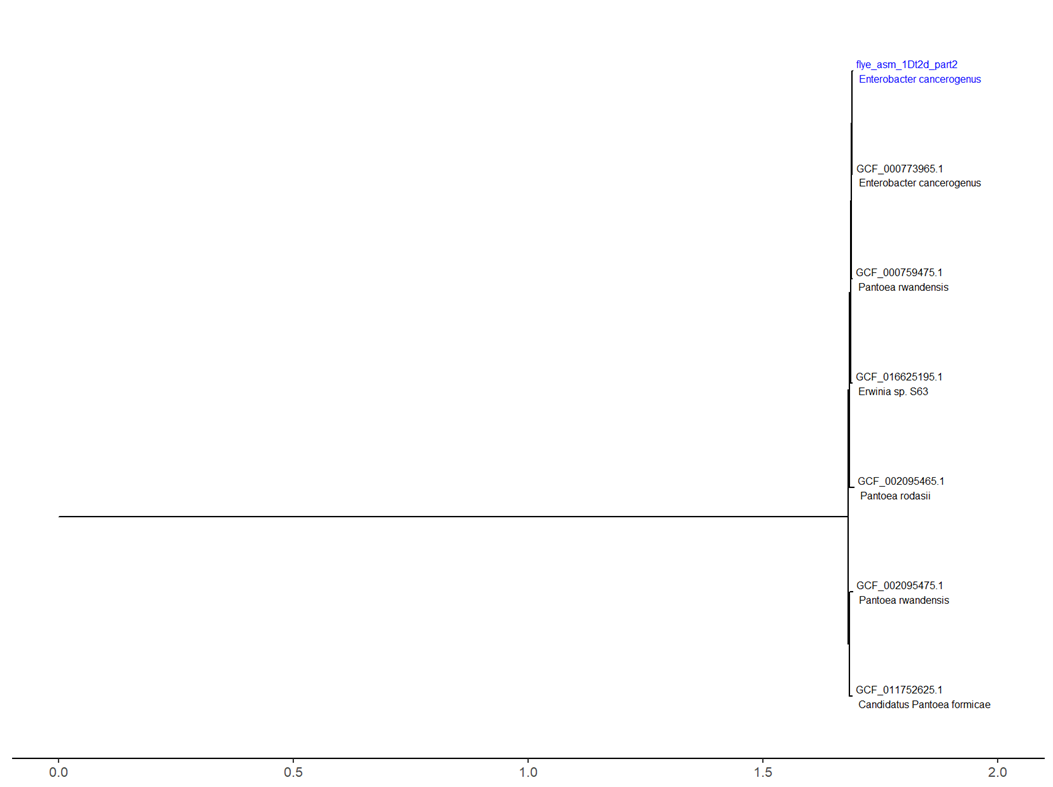
\includegraphics[width=3.51in,height=\textheight,keepaspectratio]{img/classify/classify_tree.png}

}

\caption{\label{fig-badtree}Early phylogenetic tree made using the
GTDB-Tk classify workflow}

\end{figure}%

Figure~\ref{fig-badtree} shows that the clade is not monophyletic, with
representatives from 3 genera (\emph{Enterobacter, Erwinia} and
\emph{Pantoea}).

\section{Manual trees}\label{manual-trees}

At some point I made a set of trees that cannot be sourced to any other
analysis I performed at the time.

These were made using
\href{https://github.com/aptemus/tnunn_research/blob/0c487ca21d0c783b7075446d688f88ed1d7ce77a/2024-25\%20Research/frog\%20bacteria/03\%20data_analysis/call\%20API\%20and\%20process\%20json\%20-\%20with\%20legend.R}{This
script}, which does not exist in the current version of the repo. I
cannot find what process made the basis of these trees. I remember, as
well as the small trees it output a big tree of everything that did have
them in the right place

\bookmarksetup{startatroot}

\chapter{GTDB-TK de novo}\label{gtdb-tk-de-novo}

\section{Introduction}\label{introduction-8}

£bookmark citation:
https://academic.oup.com/bioinformatics/article/36/6/1925/5626182

Earlier in the year I had used GTDB-TK to identify Genera for the 10
samples and create phylogenetic trees, this is described in
Chapter~\ref{sec-classify}. However, upon review of these trees I found
oddities, errors that did not quite make sense.

I decided to take a closer look at the
\href{https://ecogenomics.github.io/GTDBTk/index.html}{documentation}
for GTDB-TK to see what I had done exactly. I had initially used the
\href{https://ecogenomics.github.io/GTDBTk/commands/classify_wf.html?highlight=classify_wf}{classify\_wf},
it was here I discovered the
\href{https://ecogenomics.github.io/GTDBTk/commands/de_novo_wf.html}{de\_novo\_wf}.
It states:

``The \emph{de novo} workflow infers new bacterial and archaeal trees
containing all user supplied and GTDB-Tk reference genomes. The classify
workflow is recommended for obtaining taxonomic classifications, and
this workflow only recommended if a \emph{de novo} domain-specific trees
are desired. \textbf{One should take the taxonomic assignments as a
guide, but not as final classifications}. In particular, no effort is
made to resolve the taxonomic assignment of lineages composed
exclusively of user submitted genomes.''

I took this to mean that the de\_novo\_workflow would be a more accurate
way of estimating the taxonomic assignment of the samples. Though now I
re-read it I am not so sure. I found a paper that discusses this,
(\textbf{chaumeil2022?}). I then read this page,
\href{https://forum.gtdb.ecogenomic.org/t/when-should-i-use-classify-wf-instead-of-da-novo-wf/518}{on
a discussion board}. From what I understand from all of this,
Classify\_wf gives good taxonomic assignments, but its trees are not
perfect, and de\_novo\_wf is the opposite, it is weaker at assigning
(explaining why that one sample without a major group was such an error
for it) but spends more run-time making accurate trees. I shall have to
dig up my work on classify, as from what I gather, it was not an error
to run it.

\section{Methods}\label{methods-6}

The de\_novo workflow takes the .fasta files for the 10 local samples
and runs a few opperations, detailed in the documentation above, to
place them in existing trees, these are output as newick .Nexml format.
This project uses a few slurm scripts, as it is run on hawk. I produced
\href{https://github.com/tobiasnunn/tnunn_research/blob/21f2fb071d76040dc82286b9399cb11ff11a3b3c/00_scripts/de_novo_gtdbtk.sh}{this
script} to run it on hawk.

\section{Results}\label{results-5}

\section{Phylogenetic trees}\label{phylogenetic-trees}

\subsection{Introduction}\label{introduction-9}

After de\_novo\_wf analysis is done, the trees can be crafted in R.
However, it should be noted this process does not assign taxonomy to the
samples one uploads, merely places them in a tree

\subsection{Methods}\label{methods-7}

the outputs from the GTDB-tk de\_novo\_wf, namely the .nexml tree file,
can be read into R and modified to make more visually appealing, they
can then be combined with metadata to find the names, though now I see
these names may not be wholly accurate. I also toyed with the idea of
one large, interactive tree, though the capability to do that well is
beyond my current skill level. There was one sample for which a taxonomy
could not be assigned, meaning I could not isolate it to include in the
trees, thus I excluded it from further study, this perhaps was another
error on my part I now see. This is done across several scripts
£bookmark

\subsection{Results}\label{results-6}

\begin{figure}

\centering{

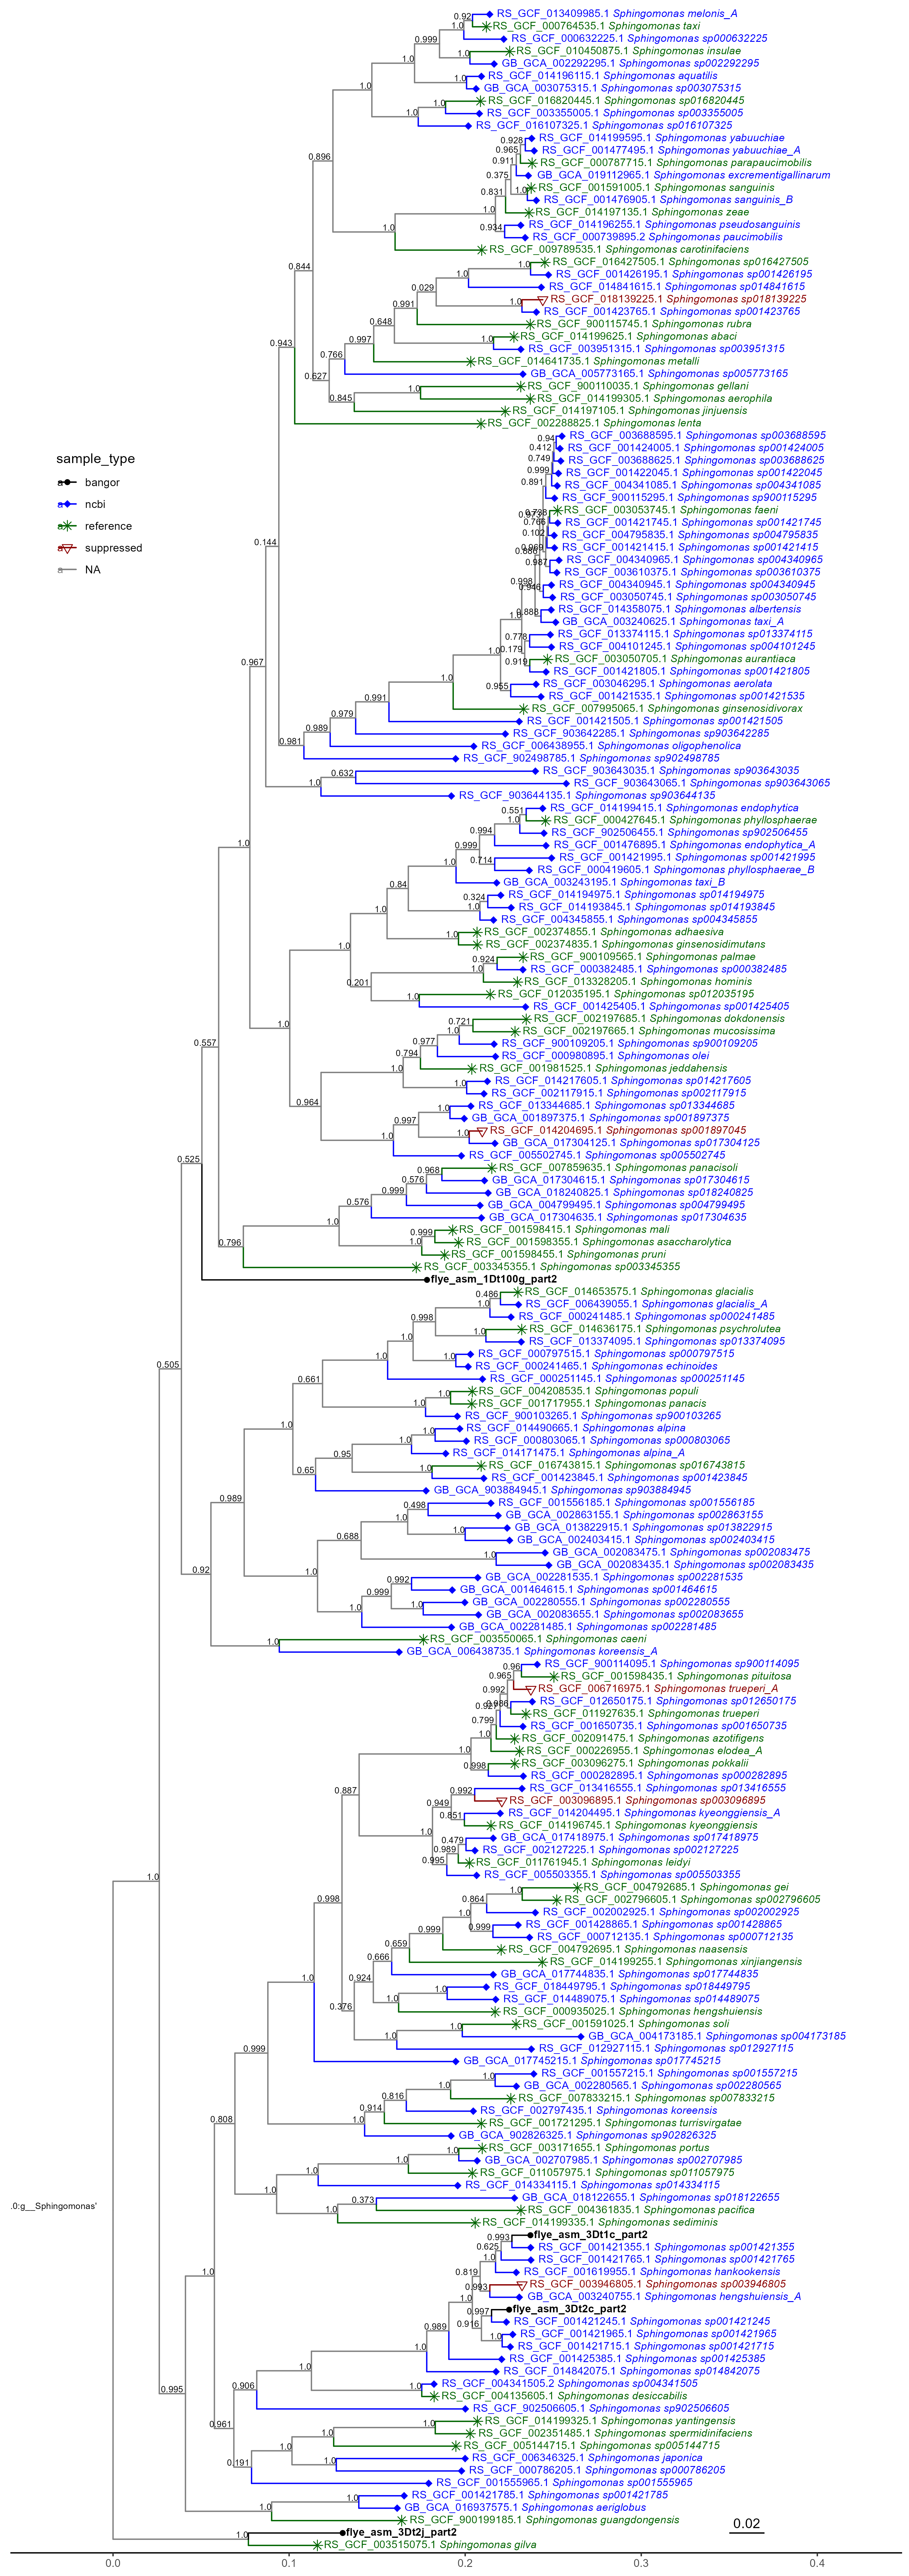
\includegraphics[width=10in,height=\textheight,keepaspectratio]{img/Sphingo_tree.png}

}

\caption{\label{fig-sphingo-tree}GTDB-tk de\_novo\_wf phylogenetic tree
for 4 Bangor-made genomic sequences in the genus \emph{Sphingomonas}
(seen in the colour black)}

\end{figure}%

\begin{figure}

\centering{

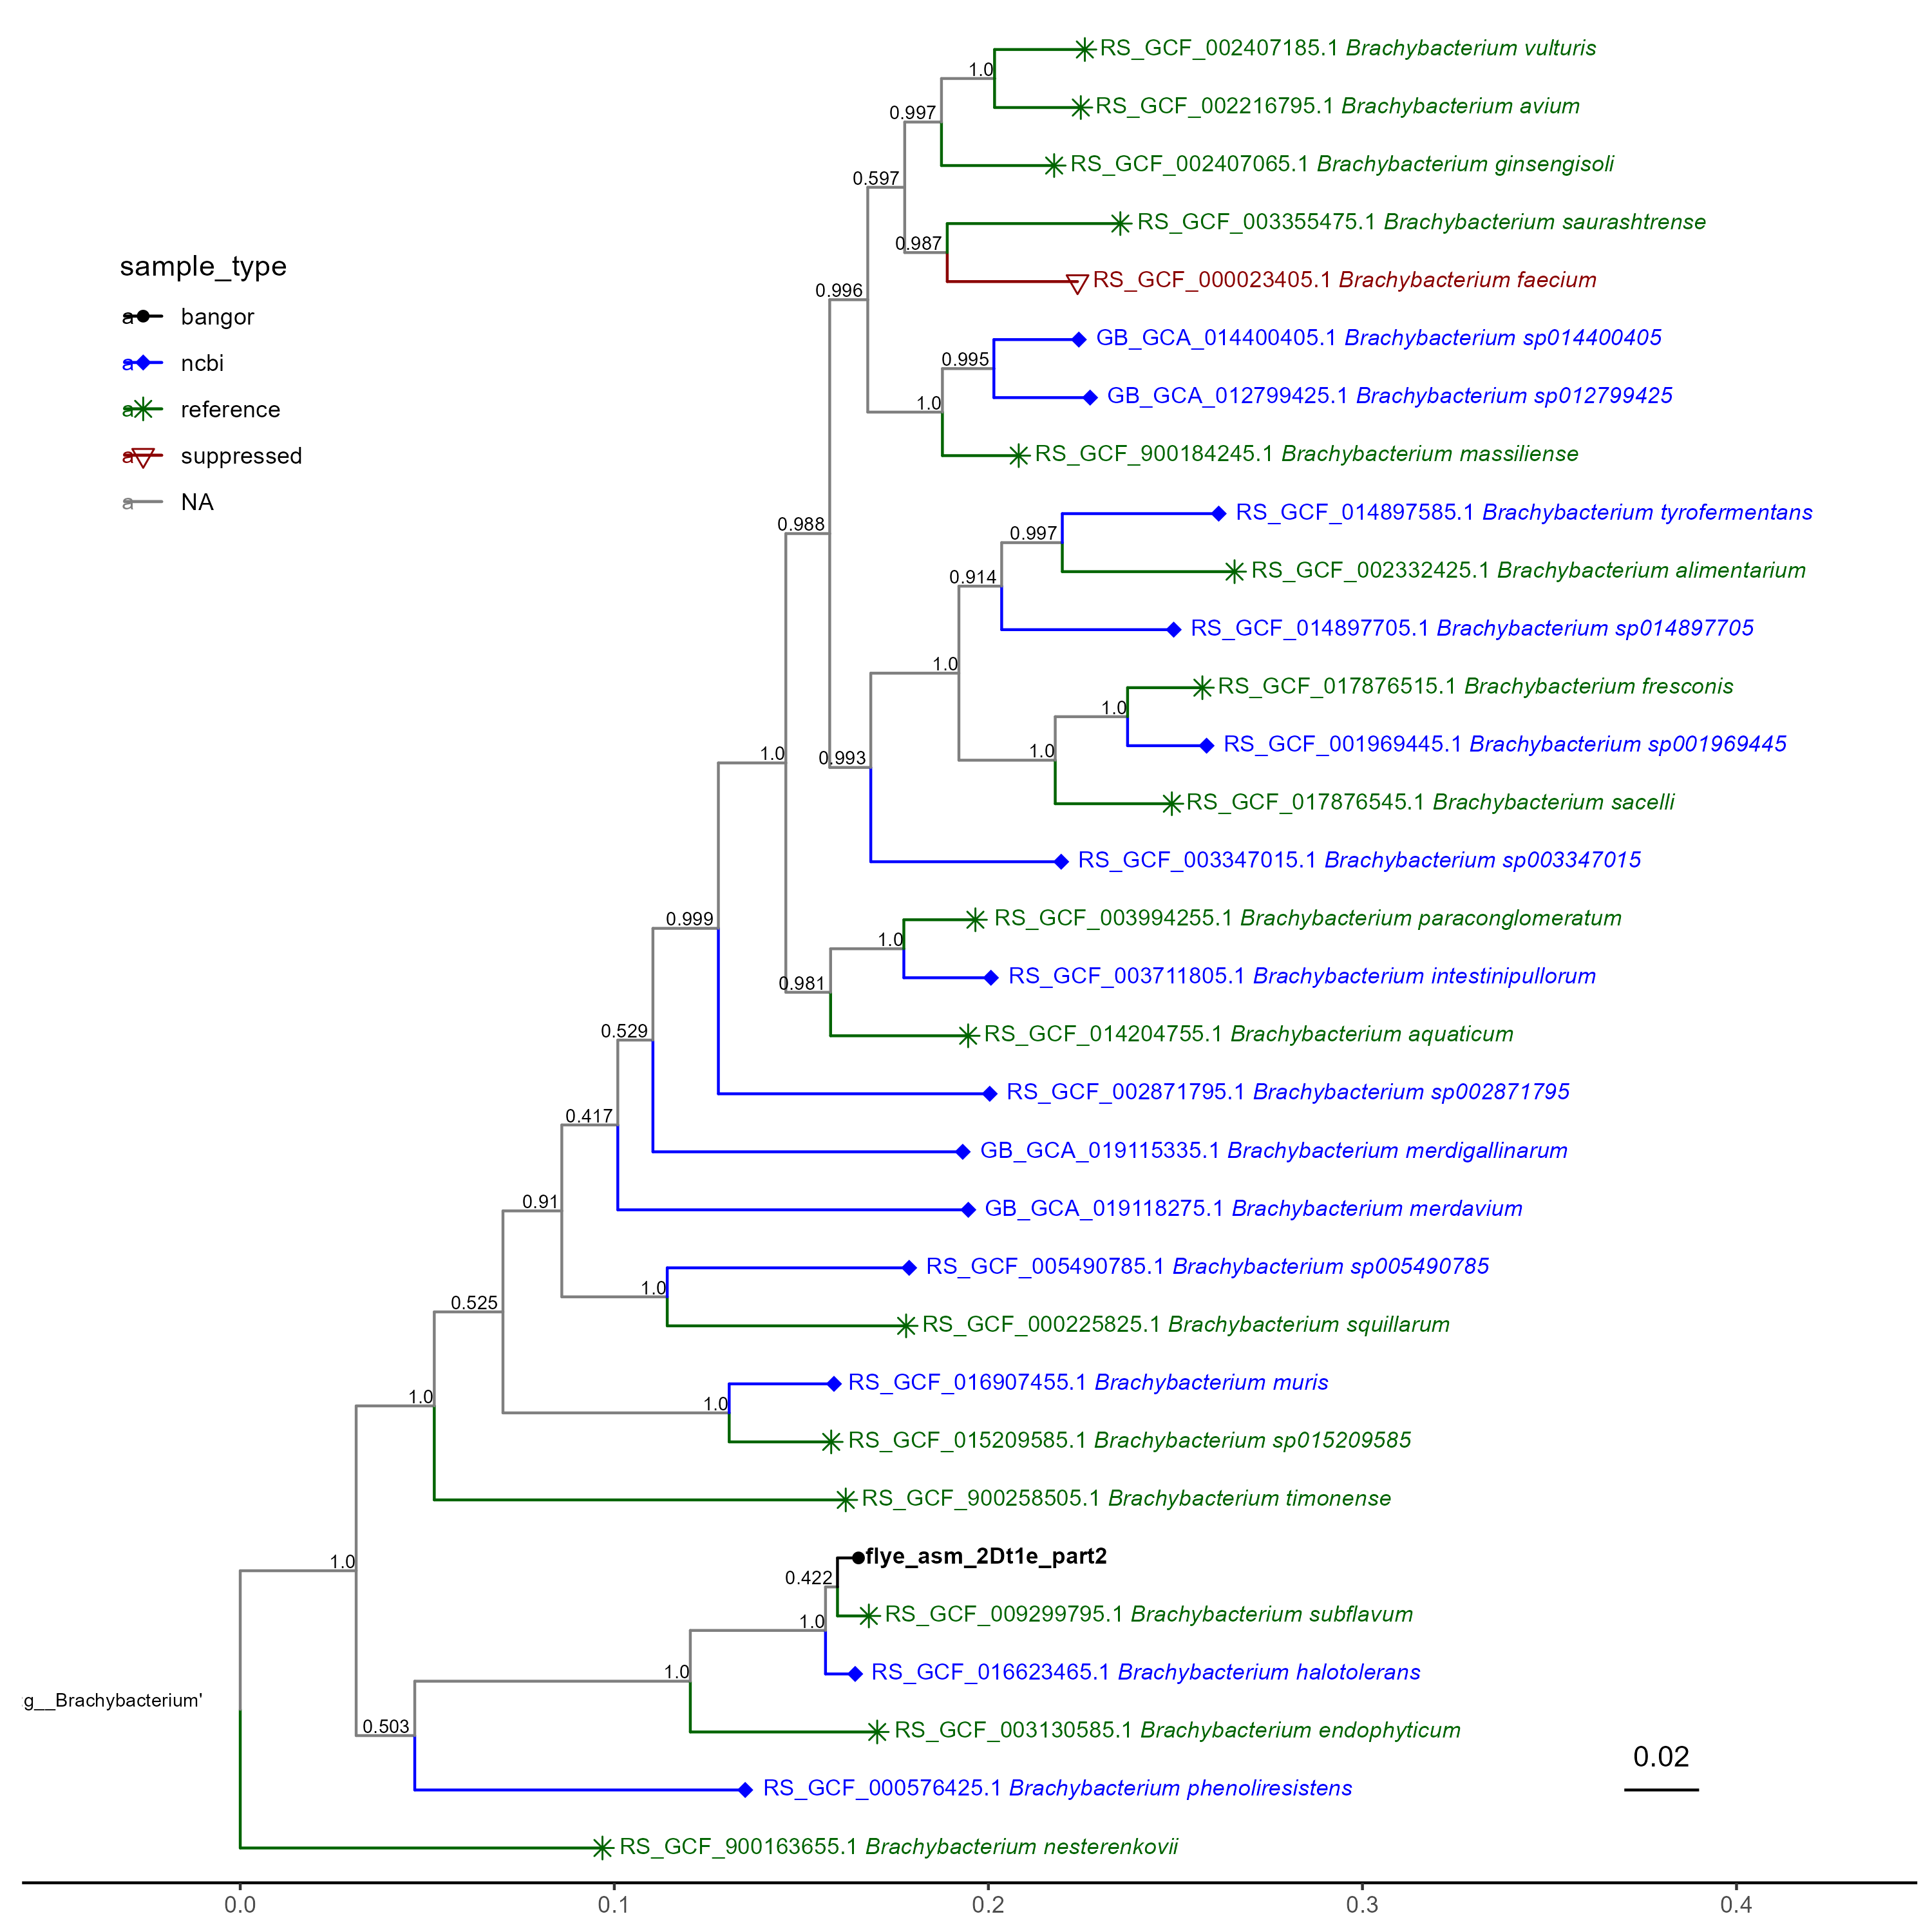
\includegraphics[width=10in,height=\textheight,keepaspectratio]{img/Brachy_tree.png}

}

\caption{\label{fig-brachy-tree}GTDB-tk de\_novo\_wf phylogenetic tree
for 1 Bangor-made genomic sequence in the genus \emph{Brachybacterium}
(seen in the colour black)}

\end{figure}%

\begin{figure}

\centering{

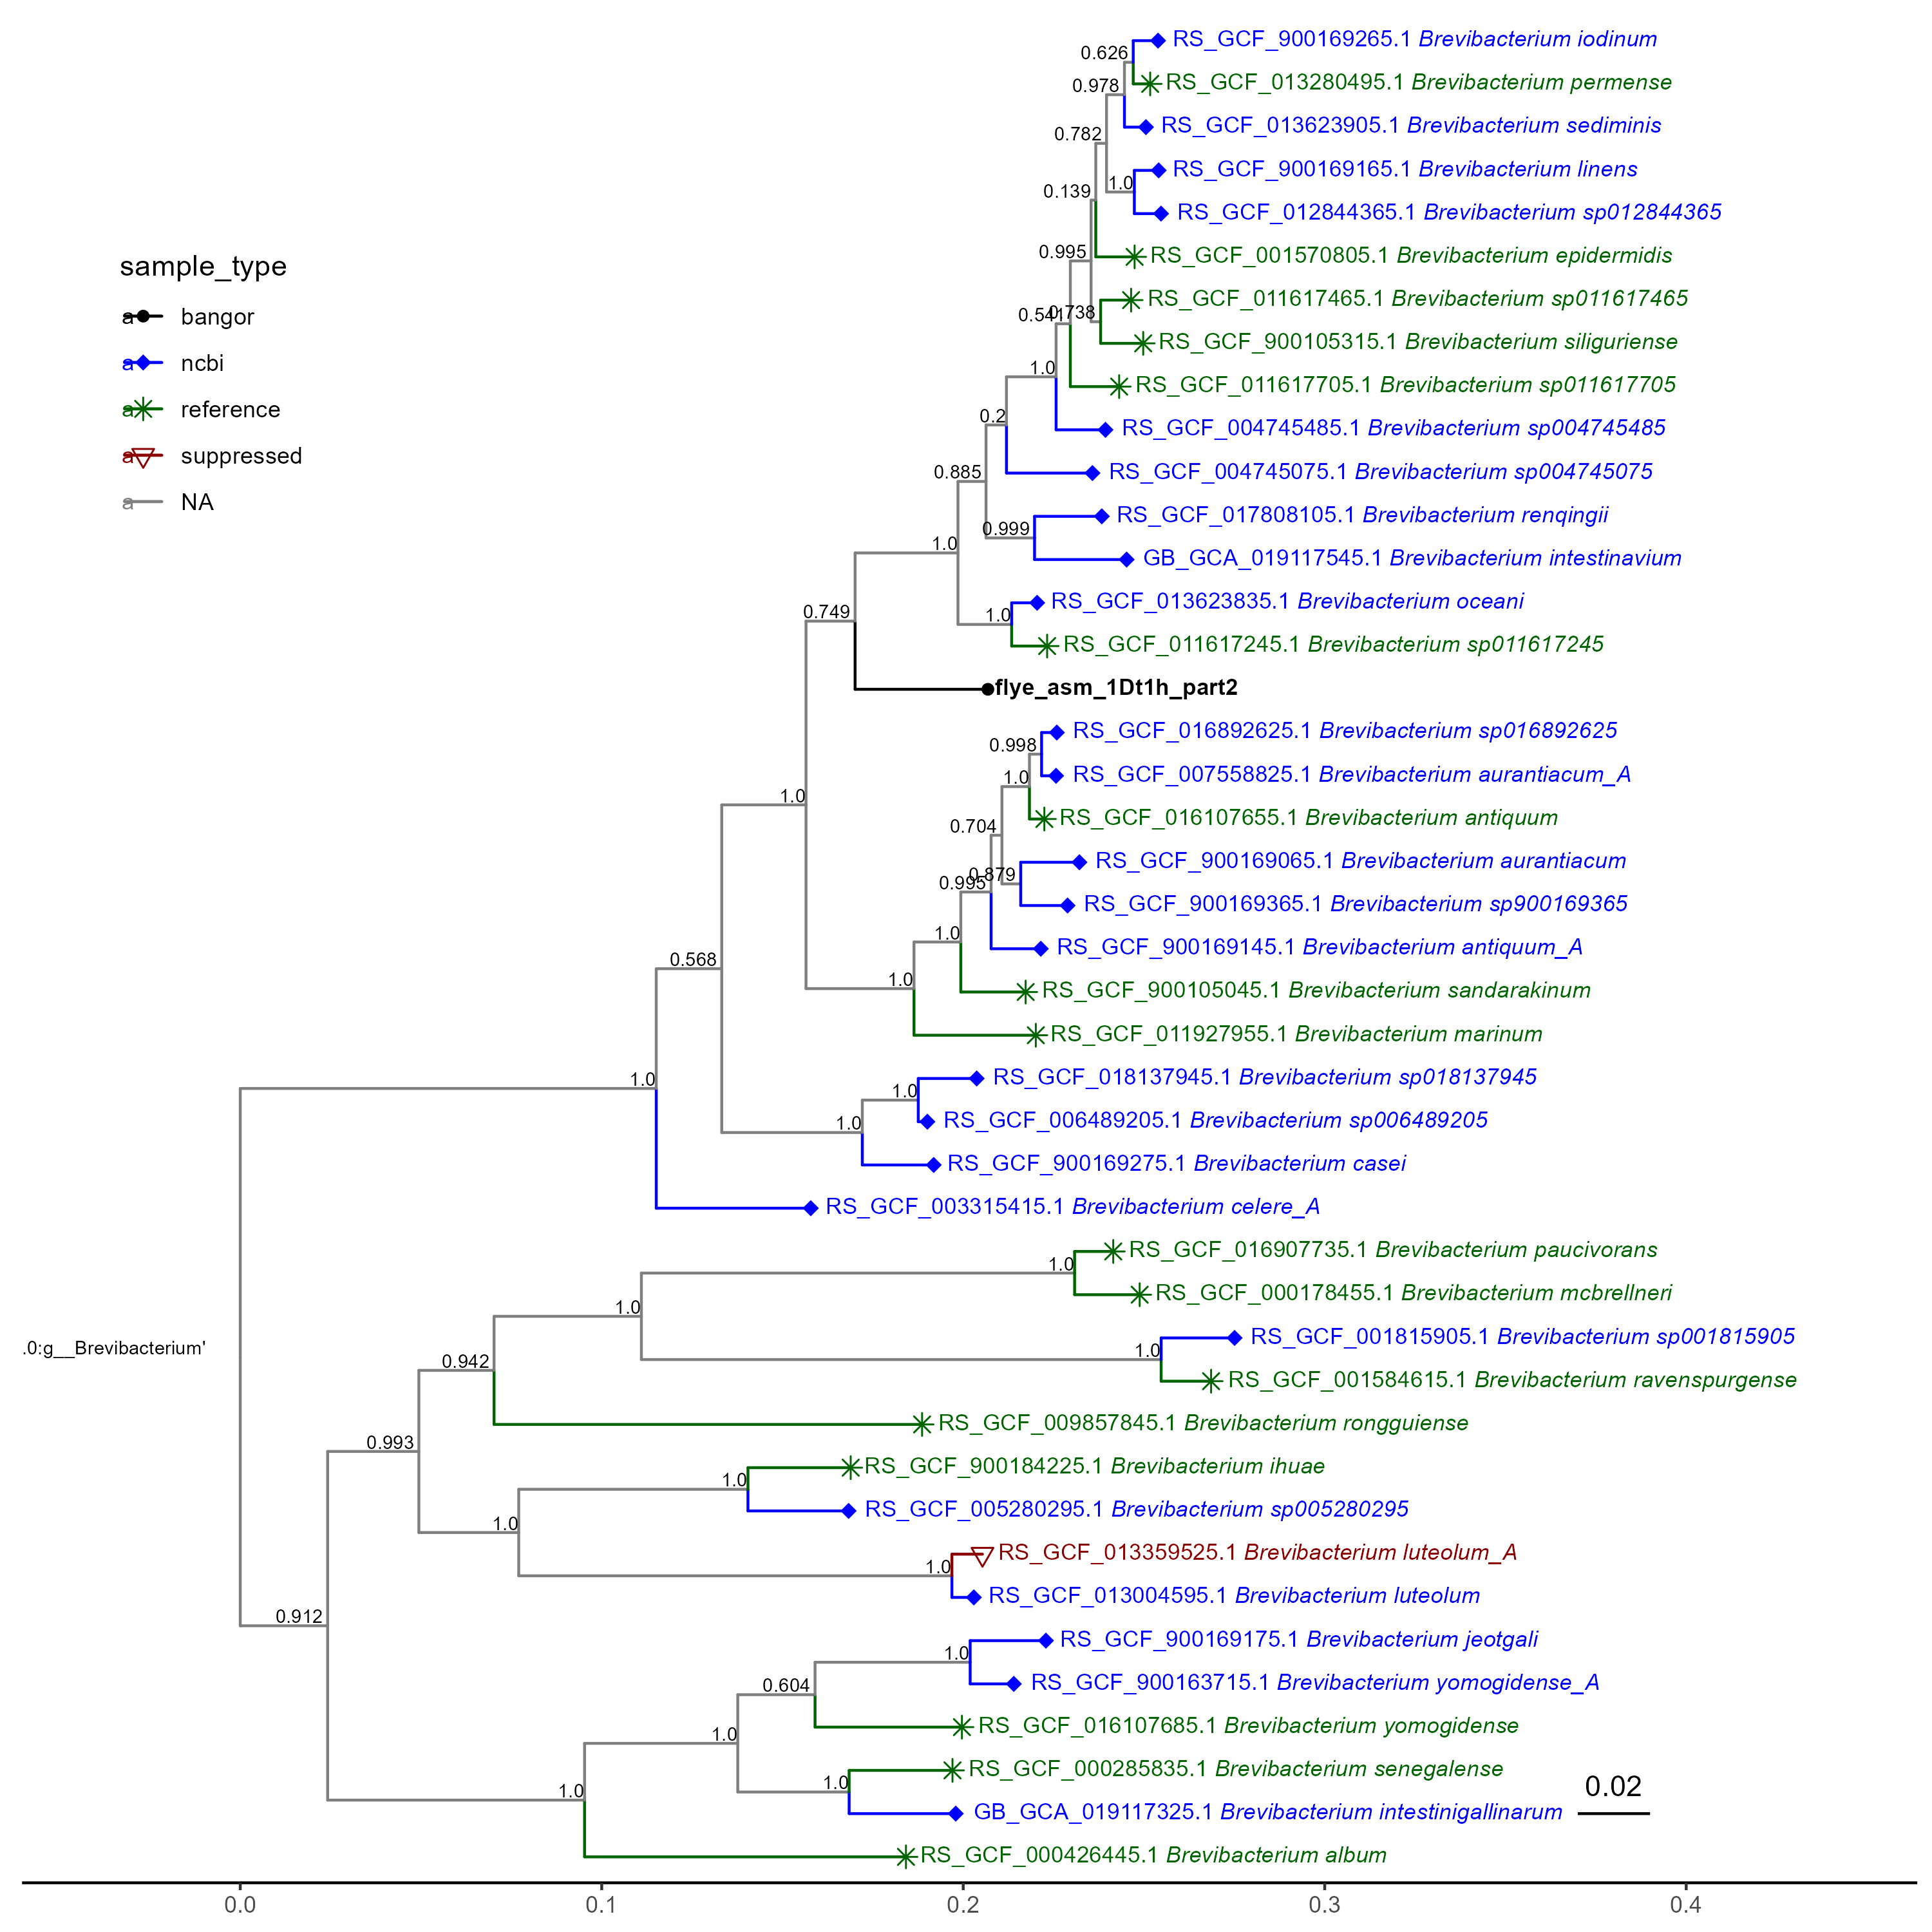
\includegraphics[width=10in,height=\textheight,keepaspectratio]{img/Brevi_tree.png}

}

\caption{\label{fig-brevi-tree}GTDB-tk de\_novo\_wf phylogenetic tree
for 1 Bangor-made genomic sequence in the genus \emph{Brevibacterium}
(seen in the colour black)}

\end{figure}%

\begin{figure}

\centering{

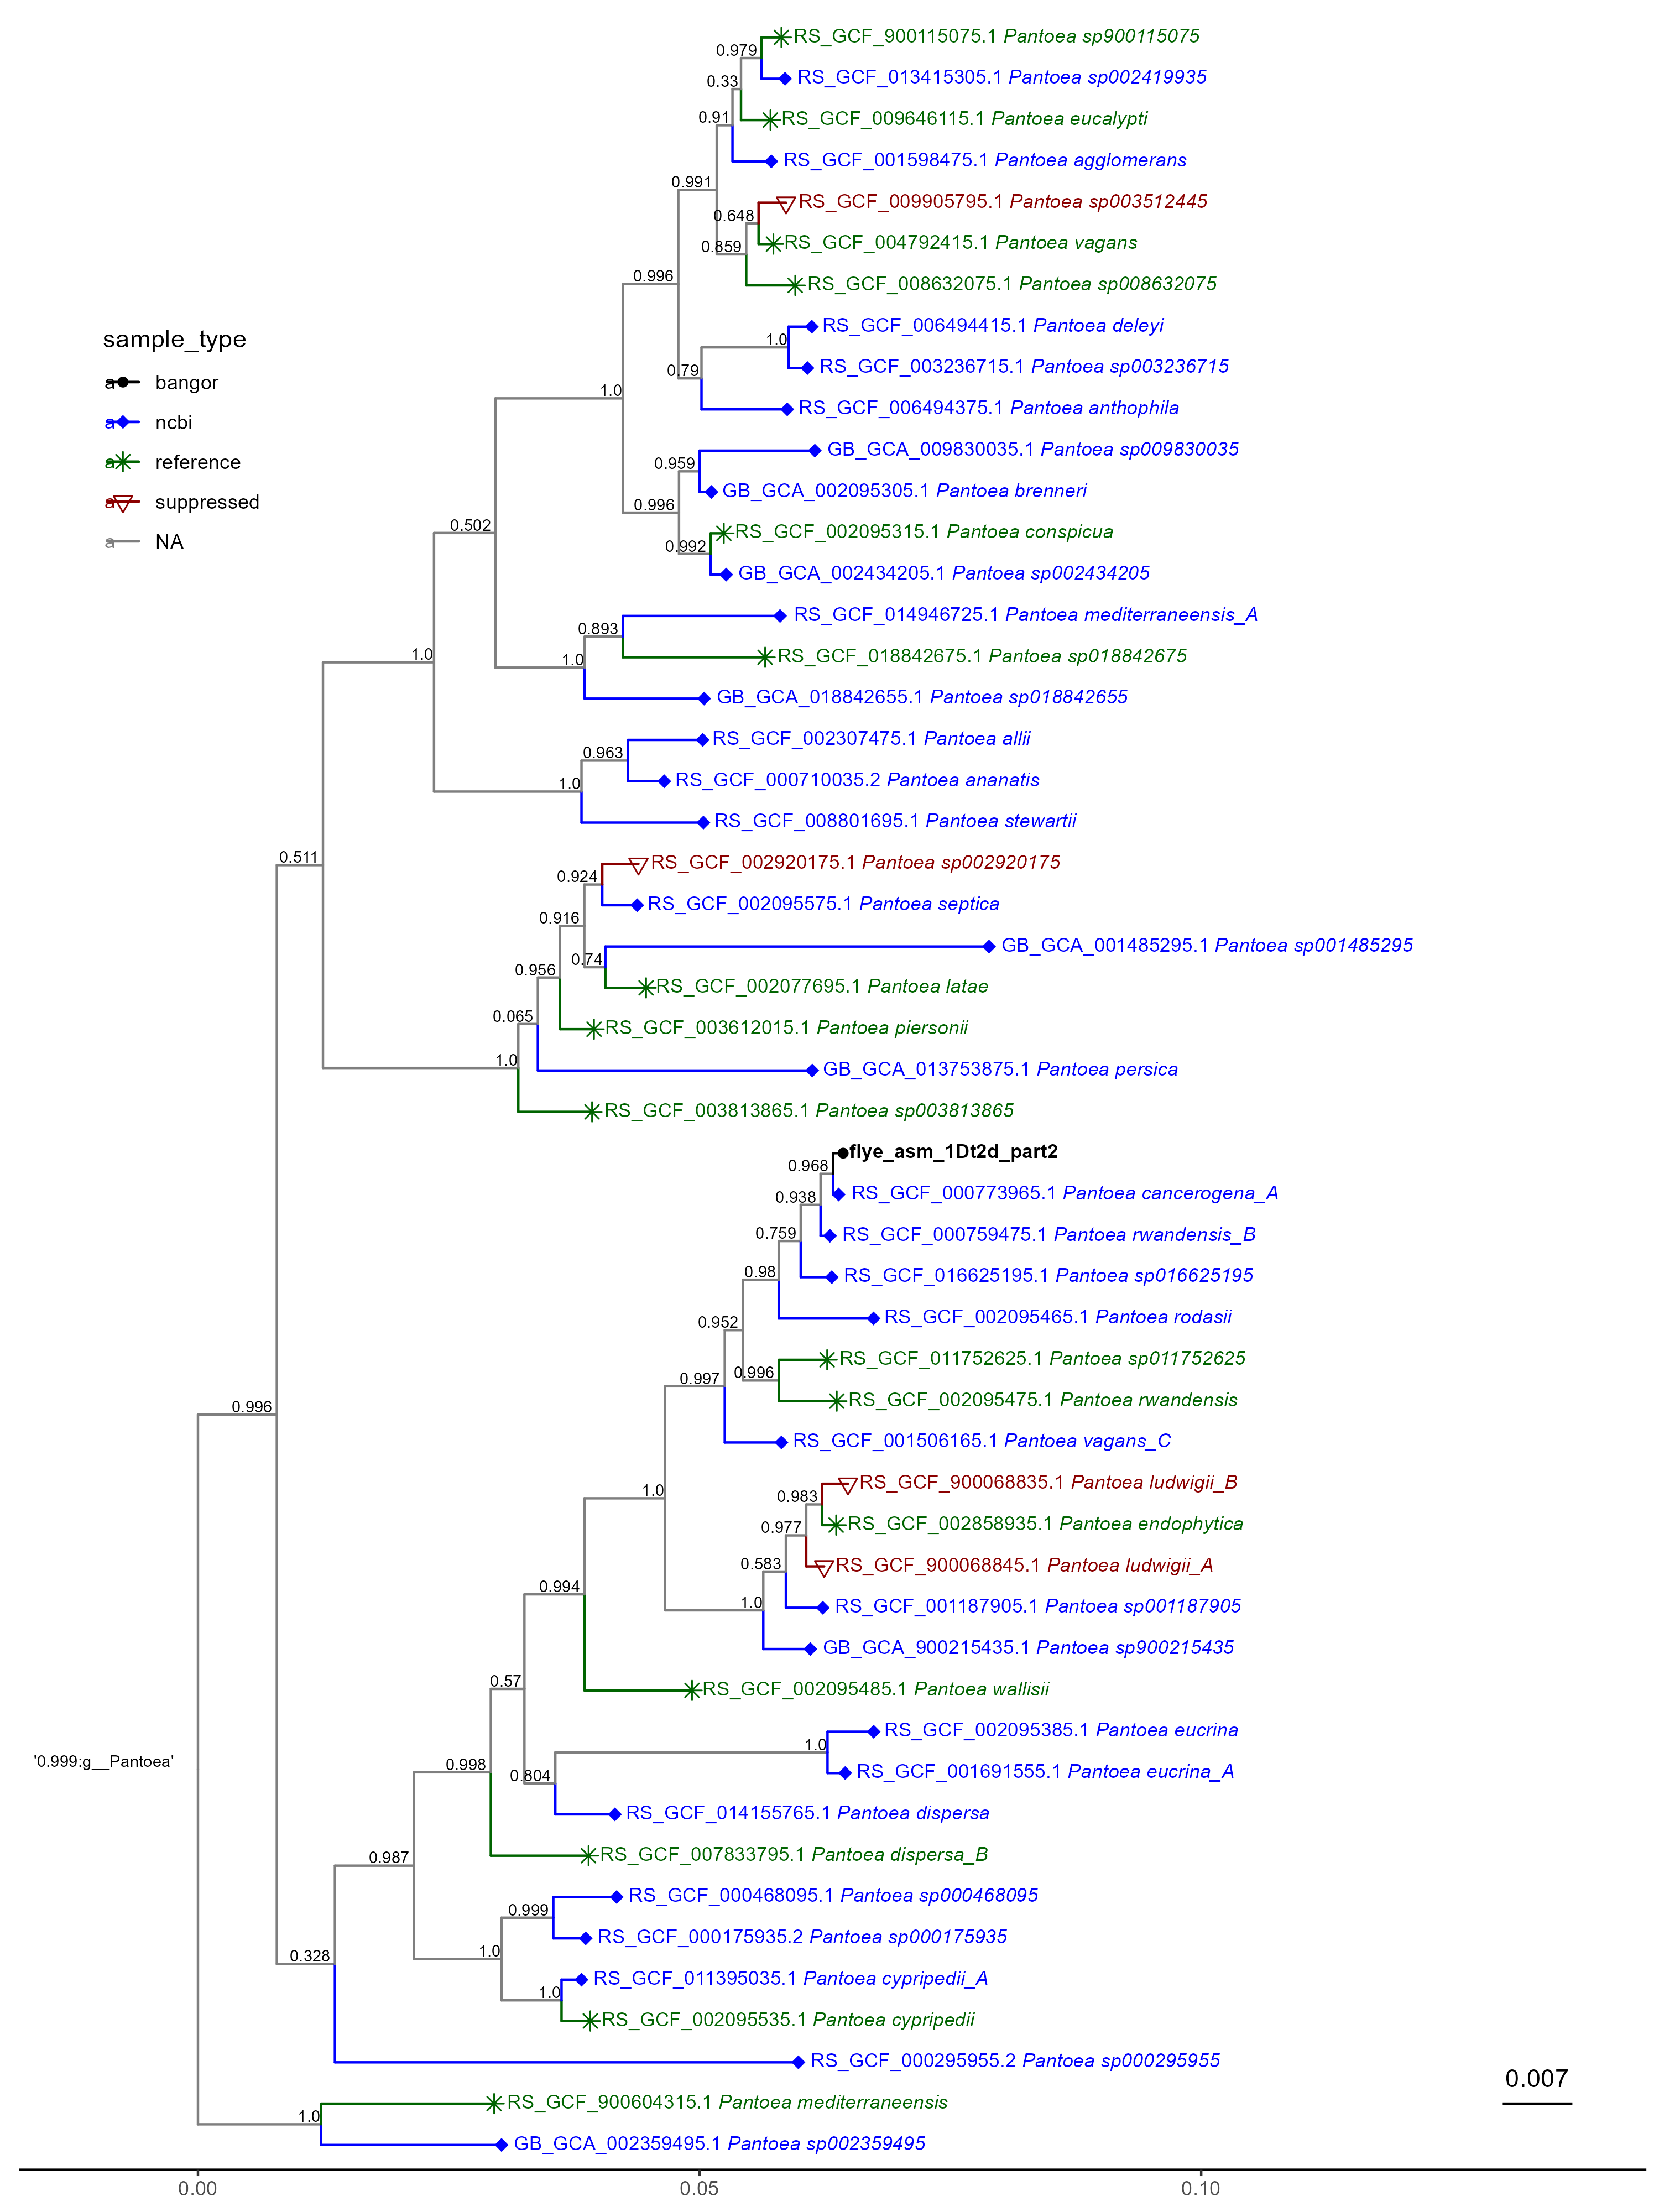
\includegraphics[width=10in,height=\textheight,keepaspectratio]{img/Panto_tree.png}

}

\caption{\label{fig-panto-tree}GTDB-tk de\_novo\_wf phylogenetic tree
for 1 Bangor-made genomic sequence of disputed genus (seen in the colour
black)}

\end{figure}%

\begin{figure}

\centering{

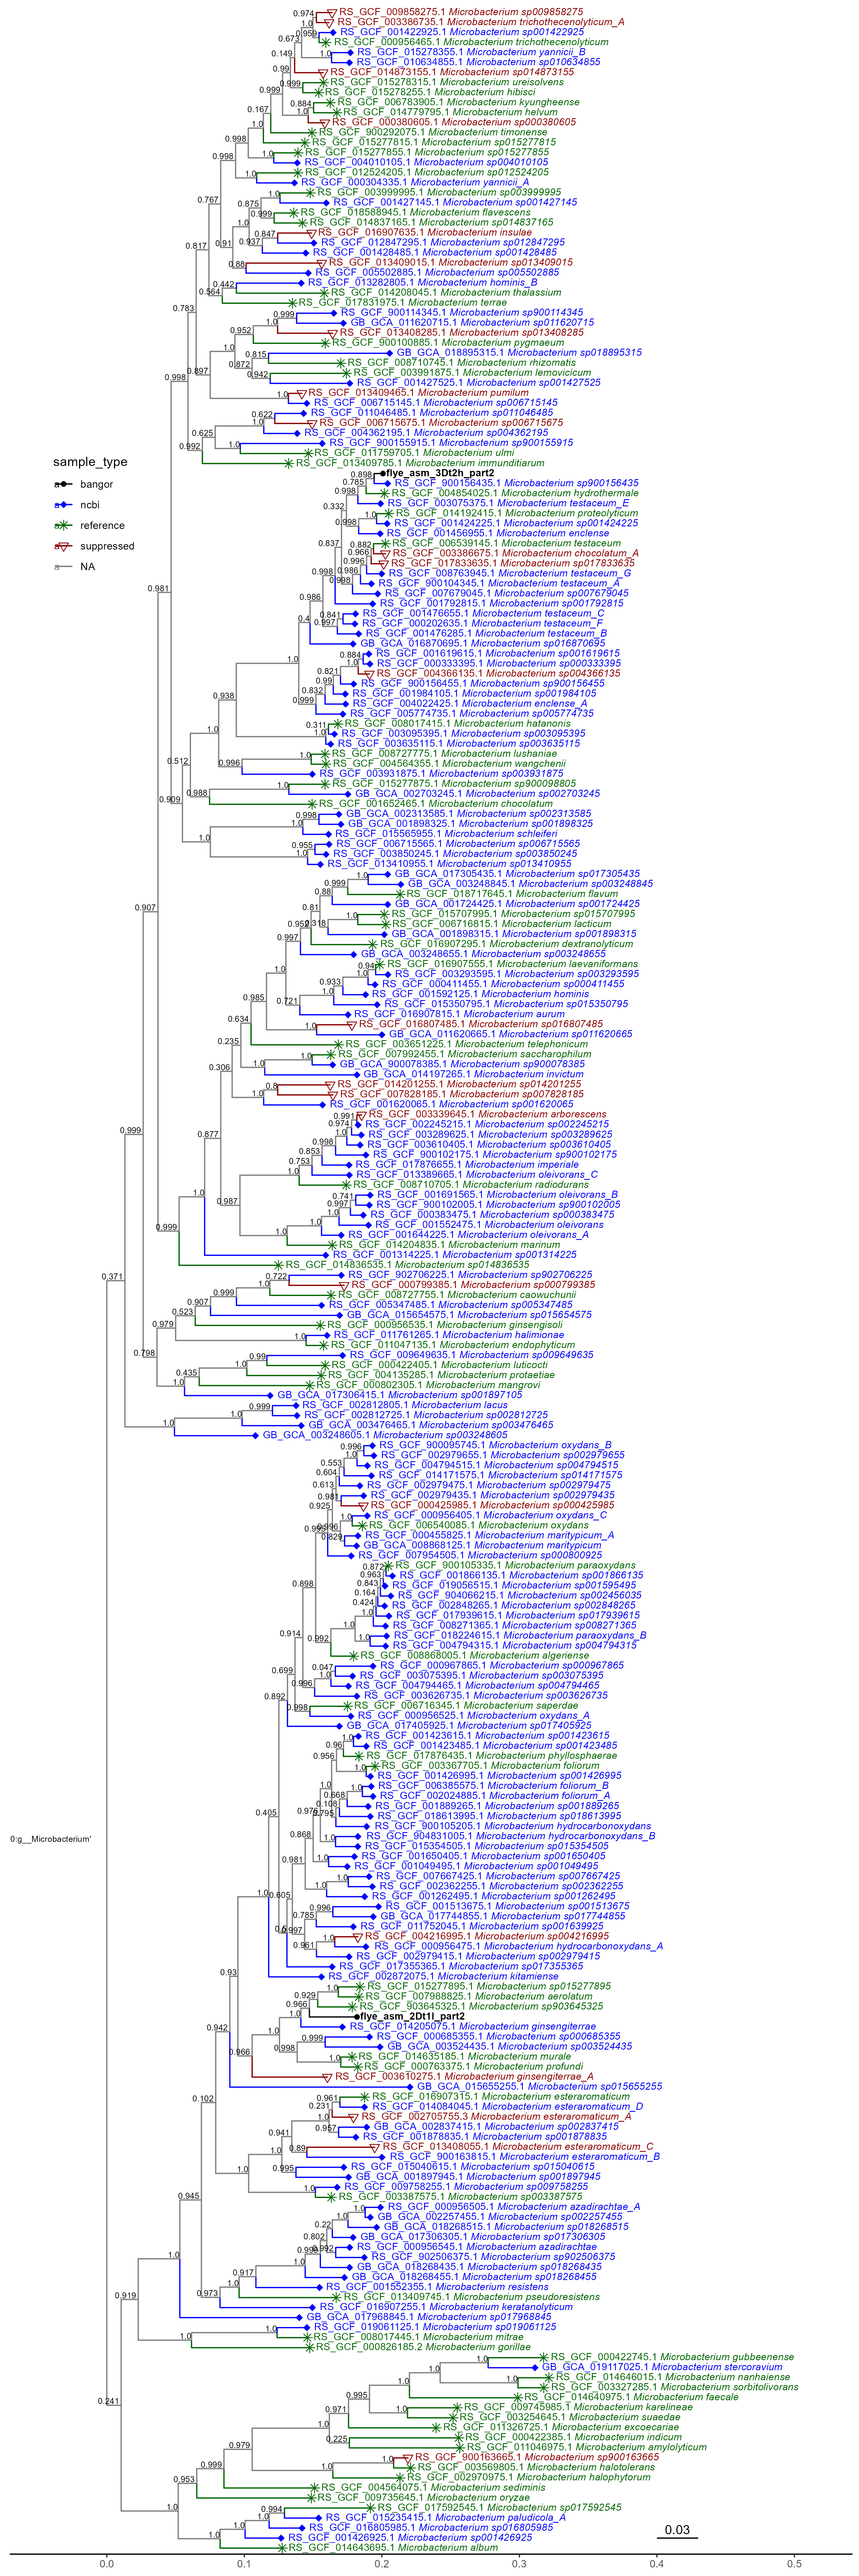
\includegraphics[width=10in,height=\textheight,keepaspectratio]{img/Micro_tree.png}

}

\caption{\label{fig-micro-tree}GTDB-tk de\_novo\_wf phylogenetic tree
for 1 Bangor-made genomic sequence of the genus \emph{Microbacterium}
(seen in the colour black)}

\end{figure}%

\section{Scripts}\label{scripts-3}

\bookmarksetup{startatroot}

\chapter{Obtaining metadata}\label{sec-ncbi}

\section{Introduction}\label{introduction-10}

Throughout the project, an understanding of the information behind the
genetic samples was important. This information was held on the same
repositories as the samples. This includes information on host,
environment, dating, sequencing method and CheckM scores for the NCBI
database, and grouping information for the KEGG database. The KEGG
metadata was especially helpful as it allows grouping boxes to be added
to the heatmaps for more transparent bioinformatics and simpler
interpretation.

\section{Methods}\label{methods-8}

API calls were used to download the metadata, they are a simple, if
technical way of transferring large quantities of data. Both the NCBI
and KEGG databases have REST APIs\footnote{REST APIs

  Here are links to both in case you want to understand them in more
  detail:

  \begin{enumerate}
  \def\labelenumi{\arabic{enumi}.}
  \item
    NCBI -
    \url{https://www.ncbi.nlm.nih.gov/datasets/docs/v2/api/rest-api/}
  \item
    KEGG - \url{https://www.kegg.jp/kegg/rest/keggapi.html}
  \end{enumerate}}. These allow communication between R and these
websites by using a special package called \texttt{httr2}, into which a
URL and other items are passed, including a list of accessions for which
data is wanted. An example of the code is used in
\href{https://github.com/tobiasnunn/tnunn_research/blob/main/Research_Experience_Module/00_scripts/Rscripts/NCBImetadatacollector.R}{NCBImetadatacollector.R}.
The code block with an indepth explanation exists in that code. In
short, one creates a list or dataframe of accessions that should be
passed to the website, so the metadata can be transferred, then several
parameters are passed in to specify what is desired, the call will then
be run and output will be several files in the .JSON format\footnote{JSON

  This is a file type that works well with API calls, it needs special
  code to unravel it and pull out the useful information into a data
  frame, but that is a topic for another section. All that is needed to
  be known here is that it is a useful filetype for online data
  transfer.}. One of the fields that needs to be passed is an output
directory.

\section{Results}\label{results-7}

\begin{figure}

\centering{

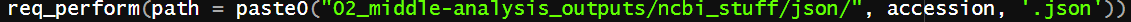
\includegraphics[width=3.77in,height=\textheight,keepaspectratio]{img/APIoutput.png}

}

\caption{\label{fig-APIcode}req\_perform method of httr}

\end{figure}%

As can be seen in Figure~\ref{fig-APIcode}, An example of having to pass
in an empty, existing directory to the call so that it can place the
data somewhere

\begin{figure}

\centering{

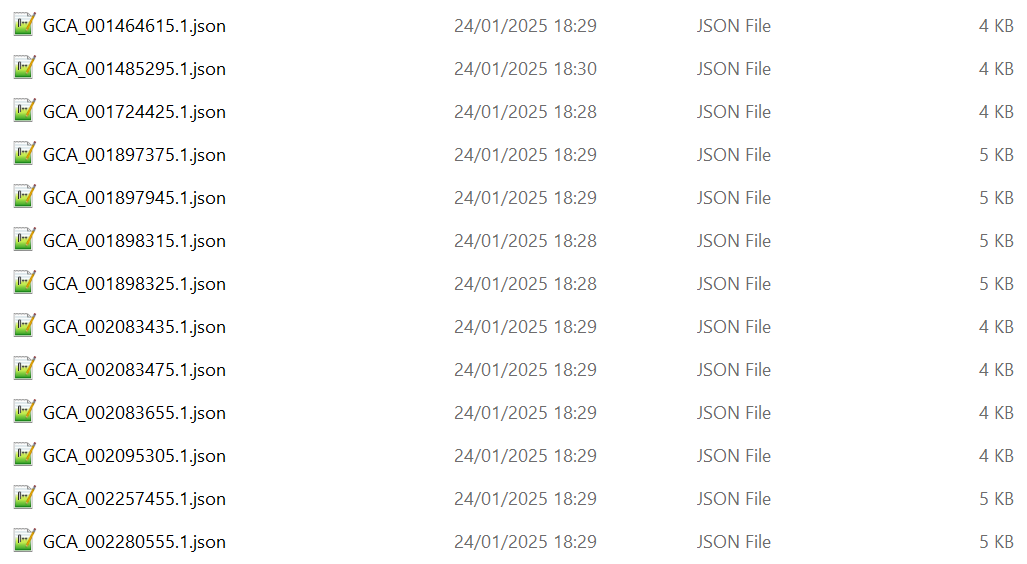
\includegraphics[width=3.42in,height=\textheight,keepaspectratio]{img/APIjsondirectory.png}

}

\caption{\label{fig-APIdirectory}JSON output from NCBI stored directly
as files}

\end{figure}%

As can be seen in Figure~\ref{fig-APIdirectory}, A subset of the files
output by my API call to illustrate what the directory would look like
on an average Windows file explorer

\section{Scripts}\label{scripts-4}

\begin{itemize}
\item
  \href{https://github.com/tobiasnunn/tnunn_research/blob/main/Research_Experience_Module/00_scripts/Rscripts/NCBI_Metadata_collector_2nd_ver.R}{NCBI\_metadata\_collector.R}
\item
  \href{https://github.com/tobiasnunn/tnunn_research/blob/main/Research_Experience_Module/00_scripts/Rscripts/NCBIfastacollector.R}{NCBI\_fasta\_collector.R}
\end{itemize}

\bookmarksetup{startatroot}

\chapter{EggNOG-mapper process - prototype}\label{sec-eggnogproto}

\section{Introduction}\label{introduction-11}

Given how long it takes to run some of the jobs, I didn't want to do all
of the eggNOG-mapper jobs before knowing if the results would be useful
and create valid heat maps at the end. So I decided to do the following:

\begin{enumerate}
\def\labelenumi{\arabic{enumi}.}
\item
  Download the metadata for the chosen genera, this used the
  \href{https://www.ncbi.nlm.nih.gov/datasets/docs/v2/api/rest-api/\#get-/genome/accession/-accessions-/dataset_report}{dataset\_report}
  API for the NCBI website. This served multiple purposes, for example
  they told me which samples have a high quality metric, they could also
  help with the generation of trees from \texttt{gtdb-tk\ de\_novo\_wf}
\item
  Choose 10 accessions per genus to use in my prototype pipeline. All
  groups totalled 10 samples, our own Bangor-made accession will be
  included in this number, excluding 1Dt100h, as \texttt{gtdb-tk} could
  not classify it into a family.
\item
  Download the genomic .fasta files for all of these. This will use the
  \href{https://www.ncbi.nlm.nih.gov/datasets/docs/v2/api/rest-api/\#get-/genome/accession/-accessions-/download}{Download
  API} to pull them from the NCBI website.
\item
  Annotate all those fastas using eggNog-mapper on hawk.
\item
  create the file(s) that turn the annotation file into a heatmap
\end{enumerate}

I chose accessions at random, ensuring there were 10 total per genus
including the Bangor samples.

All of these steps are described in more detail in
Chapter~\ref{sec-ncbi} and Chapter~\ref{sec-eggnogfull}, so instead here
I will write about the ways in which I optimised and improved the
processes before tackling the full set of 587 samples.

\section{Process Optimisation}\label{process-optimisation}

\begin{enumerate}
\def\labelenumi{\arabic{enumi}.}
\tightlist
\item
  eggNOG-mapper requires a lot of resources and can take several hours
  to complete a single job. I wanted to use the same parameters that the
  online version of eggNOG-mapper uses,
  i.e.~\texttt{-\/-evalue\ 0.001\ -\/-score\ 60\ -\/-pident\ 40\ -\/-query\_cover\ 20\ -\/-subject\_cover\ 20}
  so I didn't change them. I did change slurm parameters such as:
\end{enumerate}

\begin{itemize}
\tightlist
\item
  ntasks=2\\
\item
  cpus-per-task=25\\
\item
  time=01:00:00\\
\item
  mem=45g
\end{itemize}

After a lot of experimentation, the values above seemed to give me the
best result. I used \texttt{seff} to check I was not requesting more
resources on hawk than I needed.

\begin{enumerate}
\def\labelenumi{\arabic{enumi}.}
\setcounter{enumi}{1}
\tightlist
\item
  As the eggNOG-mapper jobs can take a long time to run, I needed a way
  to be notified when they had finished without just logging back into
  hawk. I discovered you can set mail parameters in the slurm script:
\end{enumerate}

\begin{itemize}
\tightlist
\item
  mail-user=0rtpjri2@anonaddy.me
\item
  mail-type=ALL
\end{itemize}

\begin{enumerate}
\def\labelenumi{\arabic{enumi}.}
\setcounter{enumi}{2}
\tightlist
\item
  Batching with control files You can only have 20 jobs in the queue on
  hawk at any one time, so I used a script to create `control files'.
  These contained two items per line:
\end{enumerate}

\begin{itemize}
\tightlist
\item
  the accession number
\item
  the fasta file name
\end{itemize}

I created a bash script called
\href{https://github.com/tobiasnunn/tnunn_research/blob/main/Research_Experience_Module/00_scripts/Slurmscripts/slurmsquared.sh}{slurmsquared.sh},
this script loops over the control files line by line and then executes
the slurm script
\href{https://github.com/tobiasnunn/tnunn_research/blob/main/Research_Experience_Module/00_scripts/Slurmscripts/eggnogslurmrunner.sh}{eggnogslurmrunner.sh},
passing in the accession and file name as parameters. This script
creates the slurm job to actually run eggNOG-mapper.

This way, all I had to do to process each batch of 20 was upload a new
control file and then execute slurmsquared, telling it which control
file to look at.

\begin{enumerate}
\def\labelenumi{\arabic{enumi}.}
\setcounter{enumi}{3}
\item
  Extract annotation Excel files eggNOG-mapper produces a lot of files
  but for the heatmaps I needed the Excel file which had the accession
  at the beginning and then emapper.annotations.xlsx. I created a script
  called
  \href{https://github.com/tobiasnunn/tnunn_research/blob/main/Research_Experience_Module/00_scripts/Slurmscripts/eggnog_annotation_getter.sh}{eggnog\_annotation\_getter.sh}
  to copy all the Excel files out of their main results directory into a
  separate folder, where I could download them in batches.
\item
  Separate the post-eggNOG process into different R scripts Once the KO
  values are extracted from each eggNOG-mapper annotation file, they go
  through a process in the
  \href{https://bioconductor.org/packages/devel/bioc/vignettes/microbiome/inst/doc/vignette.html}{Microbiome
  R package} called enrichKO. This takes some time to run. Separating
  out the steps into different scripts meant I didn't have to re-run the
  enrichment process but instead it could write out tsv files that I
  then used in the later steps to create the heatmap.
\end{enumerate}

The new
\href{https://github.com/tobiasnunn/tnunn_research/blob/main/Research_Experience_Module/00_scripts/Rscripts/KEGG_pipeline_pt1_enrich.R}{part1\_enrich}
focuses purely on enriching the output files and sending those outputs
into .tsv files that
\href{https://github.com/tobiasnunn/tnunn_research/blob/main/Research_Experience_Module/00_scripts/Rscripts/KEGG_pipeline_pt2_aggregate.R}{part2\_aggregate}
can now read in and aggregate, producing the output table needed in the
unmodified (but renamed)
\href{https://github.com/tobiasnunn/tnunn_research/blob/main/Research_Experience_Module/00_scripts/Rscripts/KEGG_pipeline_pt3_proportionising.R}{part3\_heatmap}.

\section{Results}\label{results-8}

The prototype phase produced the following heatmaps.

\begin{figure}

\begin{minipage}{0.50\linewidth}

\centering{

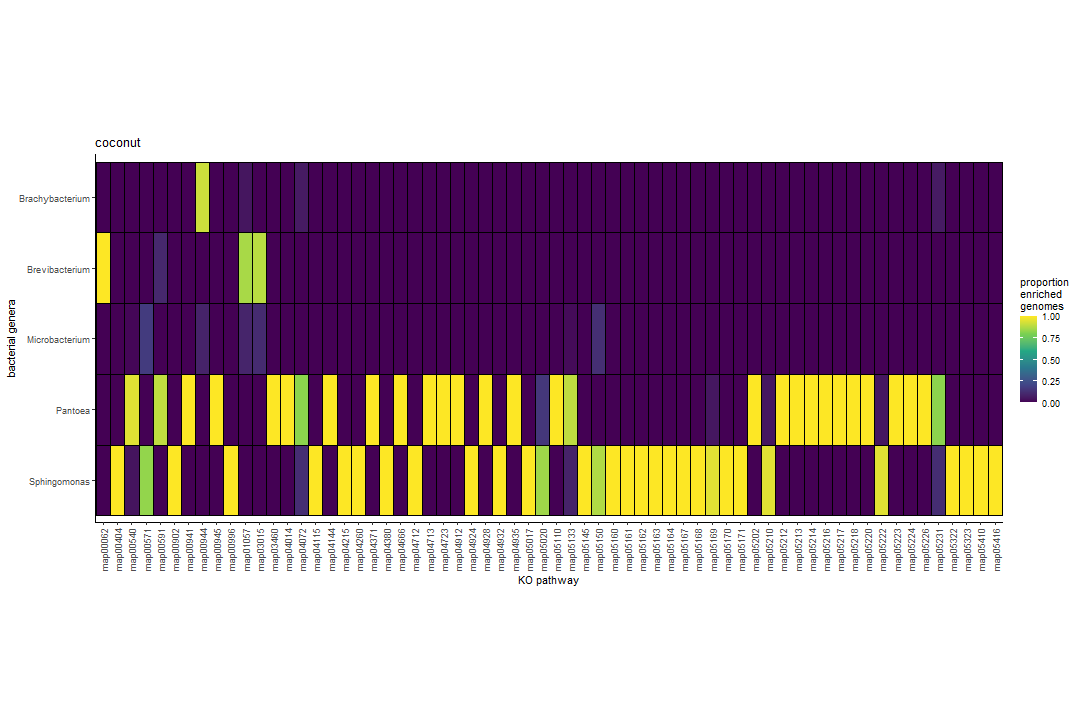
\includegraphics[width=3.6in,height=\textheight,keepaspectratio]{img/prototype_heatmaps/sample1.png}

}

\subcaption{\label{fig-protoheat-1}Aesthetic 1}

\end{minipage}%
%
\begin{minipage}{0.50\linewidth}

\centering{

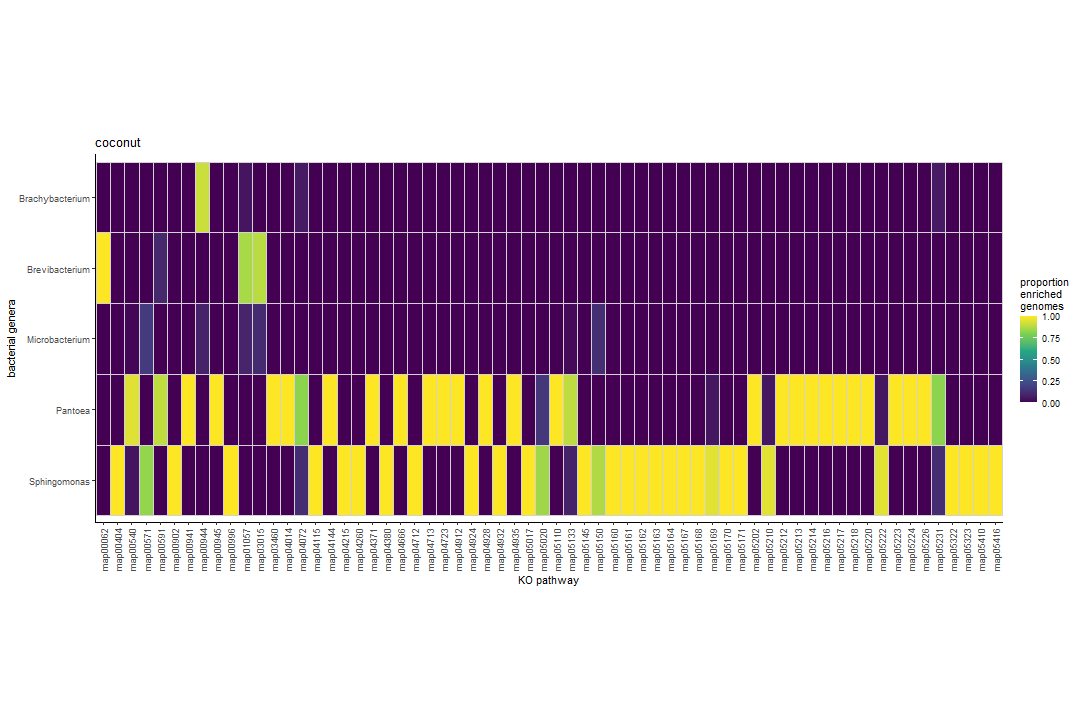
\includegraphics[width=3.6in,height=\textheight,keepaspectratio]{img/prototype_heatmaps/sample2.png}

}

\subcaption{\label{fig-protoheat-2}Aesthetic 2}

\end{minipage}%
\newline
\begin{minipage}{0.50\linewidth}

\centering{

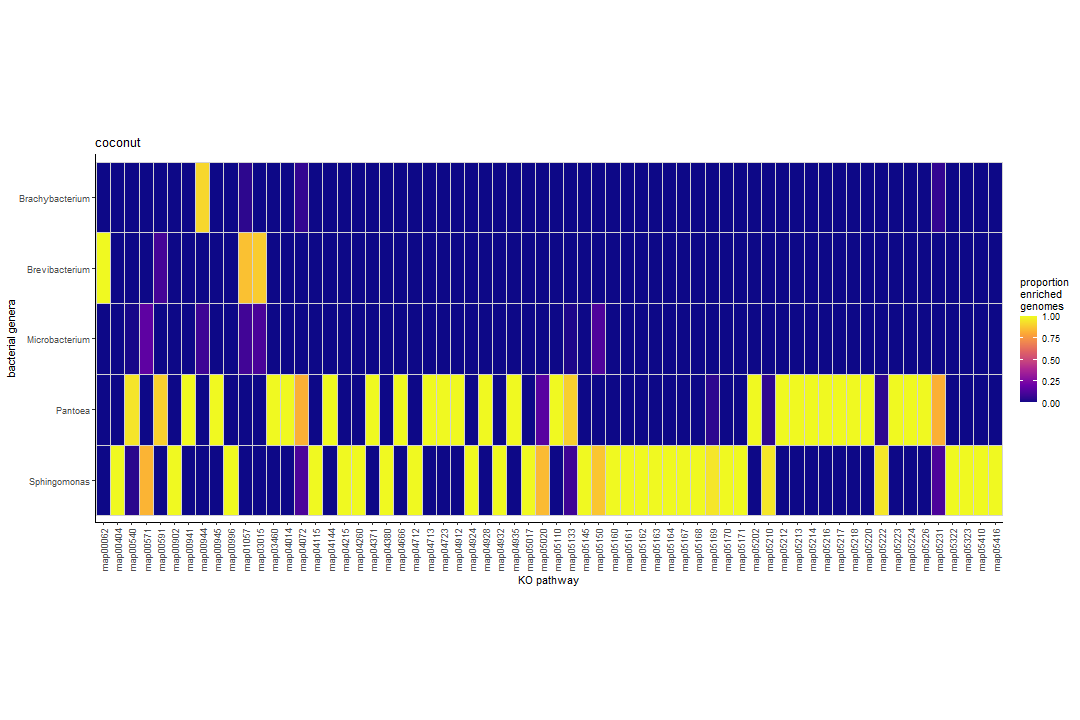
\includegraphics[width=3.6in,height=\textheight,keepaspectratio]{img/prototype_heatmaps/sample3.png}

}

\subcaption{\label{fig-protoheat-3}Aesthetic 3}

\end{minipage}%

\caption{\label{fig-protoheat}Examples of heatmaps created during
prototype phase}

\end{figure}%

\bookmarksetup{startatroot}

\chapter{eggNOG-mapper full process}\label{sec-eggnogfull}

\section{Introduction}\label{introduction-12}

Doing some stuff with eggnog

In order to create the heatmaps comparing enriched pathways, the genome
.fasta files need to be annotated\footnote{annotation

  Here meaning the process by which genes are identified from chunks of
  genome}. To do this, I used a program called EggNOG-mapper\footnote{version

  Specifically, the version on Hawk was version 2.1.12}. I had many
itterations of this process as I optimised the process through trial and
error. However, the final scripts used are: £bookmark . These scripts
are fed the .fasta files and run in slurm, outputting annotated .xlsx
format files.

\bookmarksetup{startatroot}

\chapter{Final Heatmap and analysis}\label{sec-heatmaps}

\section{Introduction}\label{introduction-13}

The main purpose of the project, this took much time to get right. The
first part of the process is discussed above. This section concerns the
output of EggNOG-mapper, which become the inputs here, with the end goal
of creating a heatmap where 1 Genus has over 80\% of accessions enriched
for a pathway and each of the others have less than 20\%. This task
created a pipeline that evolved over time, but the current scripts that
are used are:

\begin{enumerate}
\def\labelenumi{\arabic{enumi}.}
\item
  \href{https://github.com/tobiasnunn/tnunn_research/blob/09b6d09dd31e29cd56289794bffb23397e7baf15/Research_Experience_Module/00_scripts/Rscripts/KEGG_pathway_pipeline_p1_enrich.R}{KEGG\_pathway\_pipeline\_p1\_enrich.R}
\item
  \href{https://github.com/tobiasnunn/tnunn_research/blob/09b6d09dd31e29cd56289794bffb23397e7baf15/Research_Experience_Module/00_scripts/Rscripts/KEGG_pathway_pipeline_p2_aggregate.R}{KEGG\_pathway\_pipeline\_p2\_aggregate.R}
\item
  \href{https://github.com/tobiasnunn/tnunn_research/blob/09b6d09dd31e29cd56289794bffb23397e7baf15/Research_Experience_Module/00_scripts/Rscripts/KEGG_pathway_pipeline_p3_proportion.R}{KEGG\_pathway\_pipeline\_p3\_proportion.R}
\end{enumerate}

These are in specifically that order, as one file feeds the next.

\section{Methods}\label{methods-9}

Once the output of EggNOG-mapper is downloaded
(\textbf{?@sec-eggnogmapper}), they must first be enriched. This is p1
of the pipeline
\href{https://github.com/tobiasnunn/tnunn_research/blob/09b6d09dd31e29cd56289794bffb23397e7baf15/Research_Experience_Module/00_scripts/Rscripts/KEGG_pathway_pipeline_p1_enrich.R}{KEGG\_pathway\_pipeline\_p1\_enrich.R}.
The R package \texttt{Mircrobiomeprofiler} is used, specifically the
\texttt{EnrichKO()} function to itterate over all the annotated
accessions.

However, having a couple thousand individual enriched files cannot make
a heatmap, thus they must be aggregated into one file,
\href{https://github.com/tobiasnunn/tnunn_research/blob/09b6d09dd31e29cd56289794bffb23397e7baf15/Research_Experience_Module/00_scripts/Rscripts/KEGG_pathway_pipeline_p2_aggregate.R}{KEGG\_pathway\_pipeline\_p2\_aggregate.R}.

Finally, the proportions must be applied to this so that only the rows
meeting the criteria (\textgreater80\% in any one and \textless20\% in
the rest),
\href{https://github.com/tobiasnunn/tnunn_research/blob/09b6d09dd31e29cd56289794bffb23397e7baf15/Research_Experience_Module/00_scripts/Rscripts/KEGG_pathway_pipeline_p3_proportion.R}{KEGG\_pathway\_pipeline\_p3\_proportion.R}.
I merged a 4th script with this, so this one also contains all of the
formatting for the heatmap.

\section{Results}\label{results-9}

\begin{figure}

\centering{

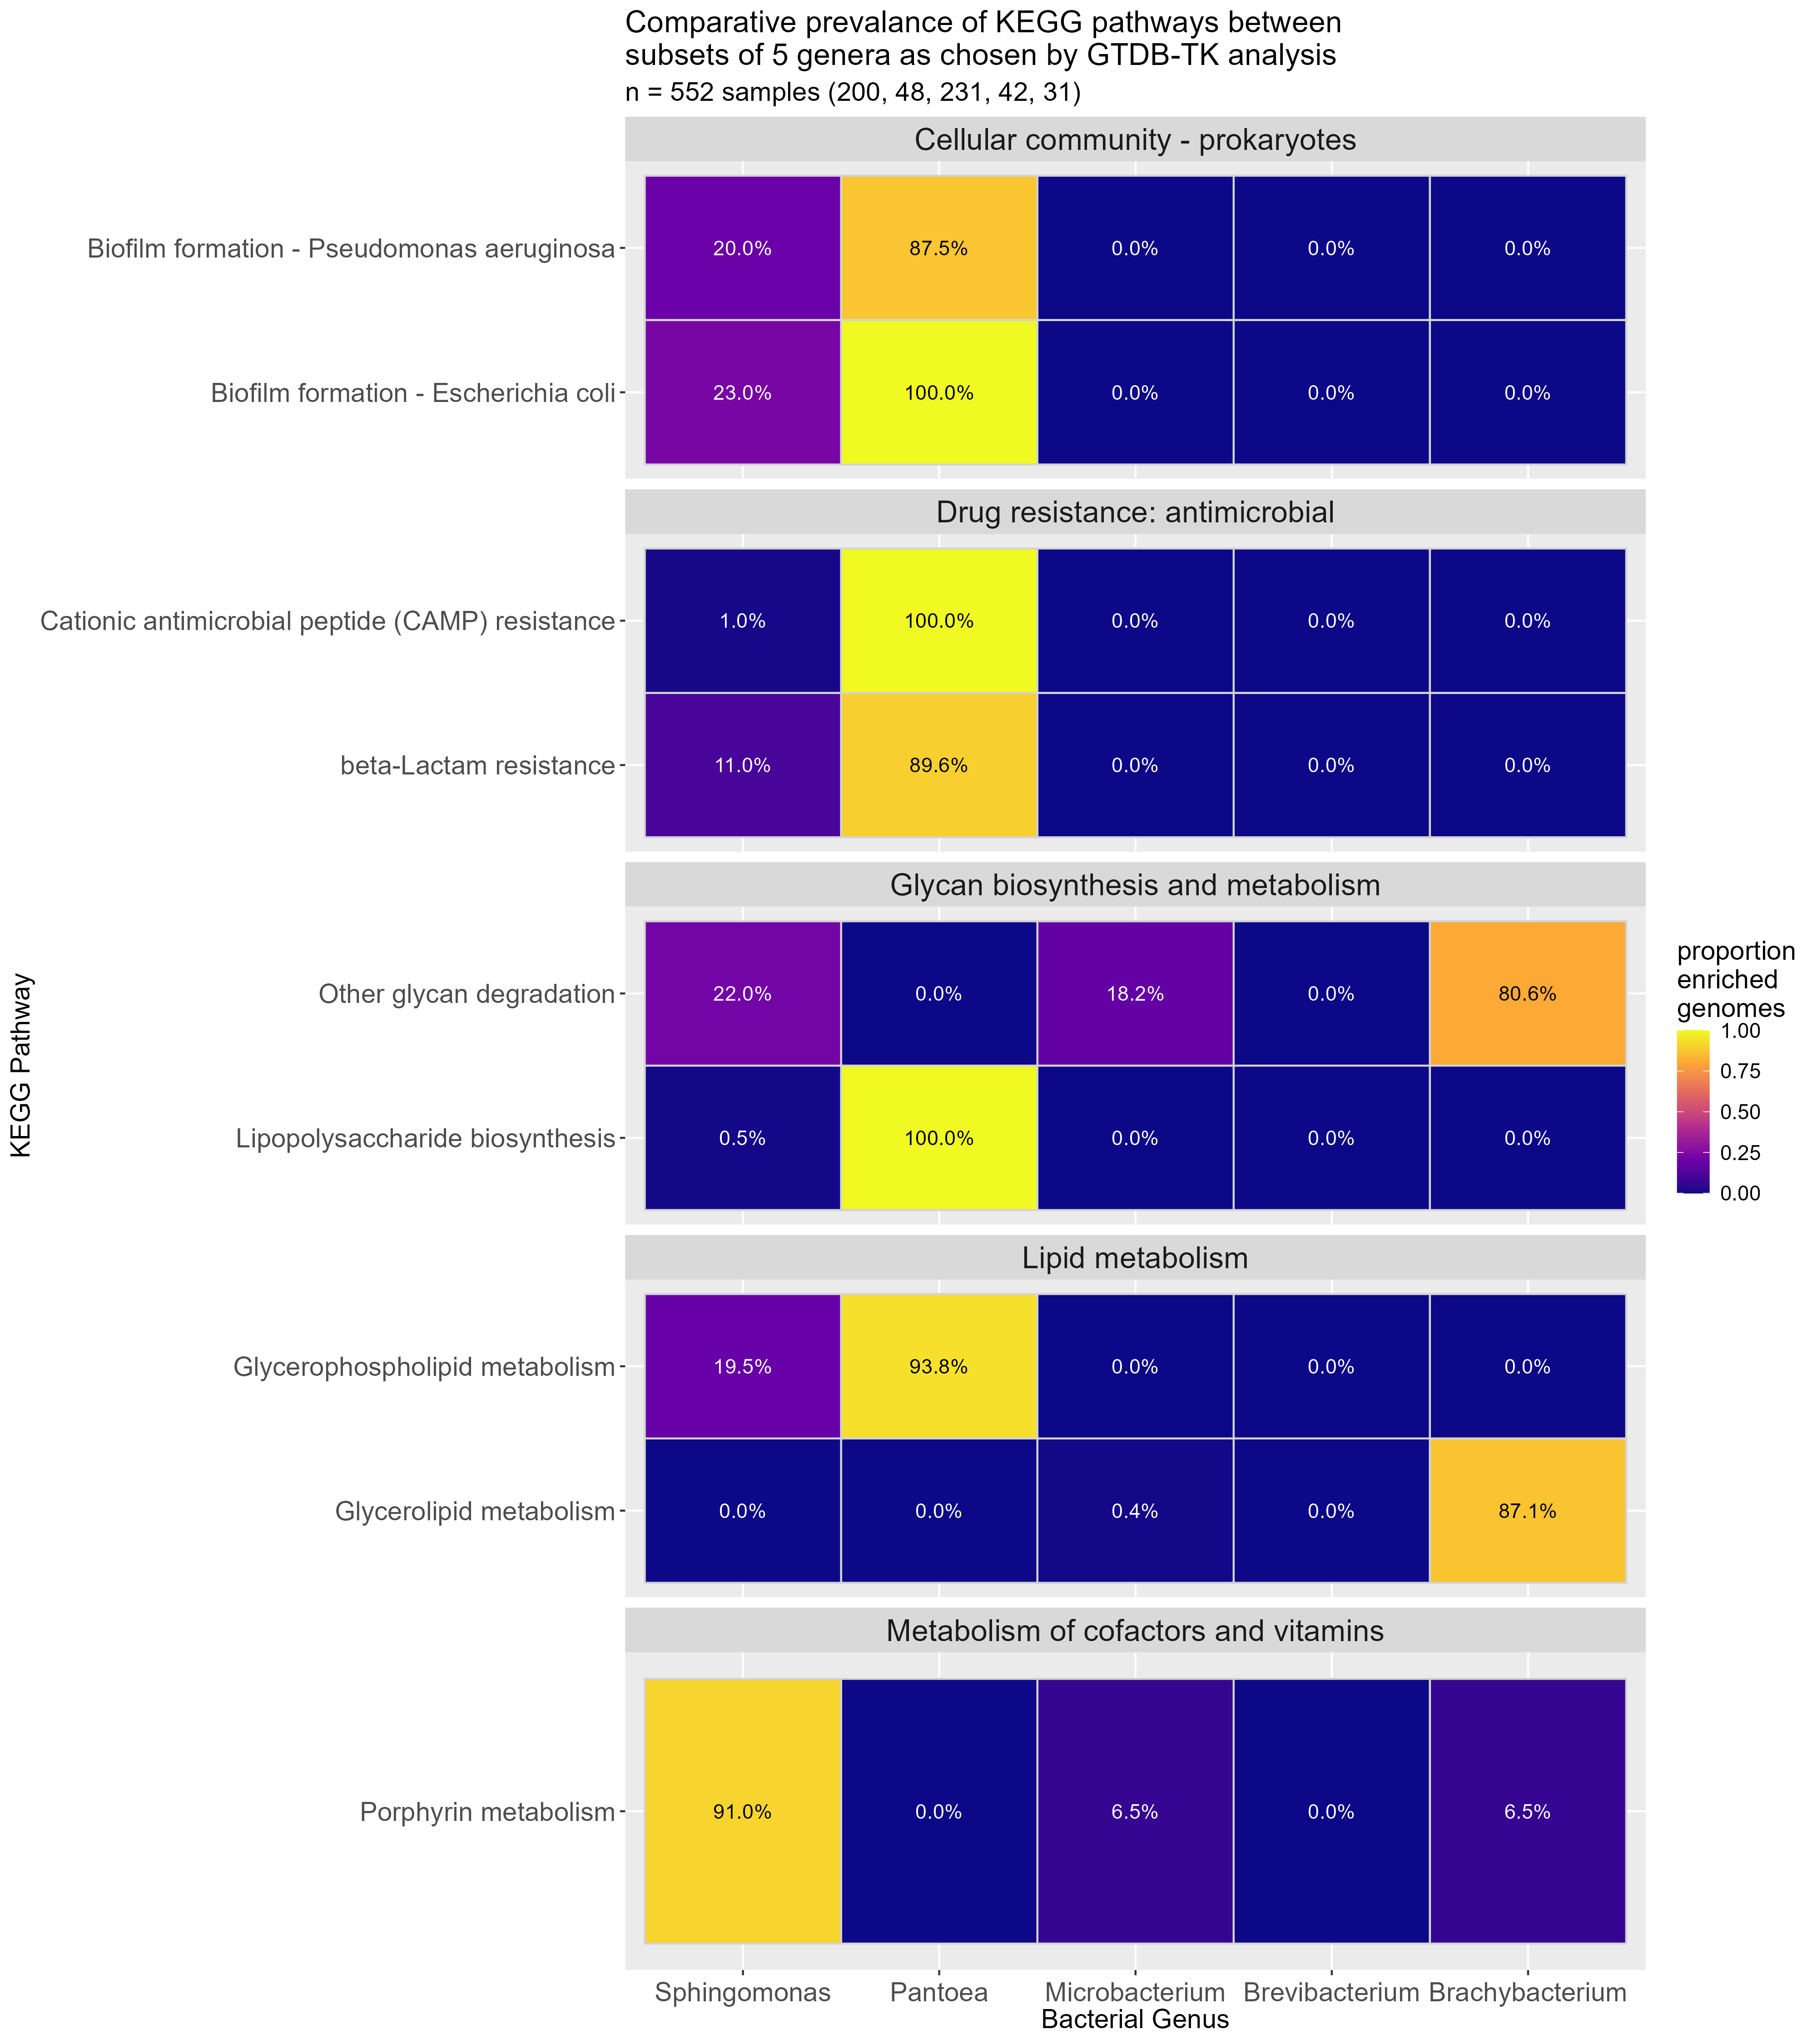
\includegraphics[width=13.33in,height=\textheight,keepaspectratio]{img/all_genera_updated_b.png}

}

\caption{\label{fig-final-heatmap}Heatmap comparing significant map
pathways in 552 samples of both laboratory and public origin}

\end{figure}%

As can be seen in Figure~\ref{fig-final-heatmap}, metabolism makes up
three of the five KEGG groupings. Seen to be more enriched in one Genus
than the others. With the other two being Drug resistence and biofilm
formation. The Genus \emph{Pantoea} makes up 6 of the 9 pathways found,
with \emph{Microbacterium} and \emph{Brevibacterium} having none.

\section{Next steps}\label{next-steps}

other heatmaps like the common one, the cutdown one

link to the prototype page where i did those

\bookmarksetup{startatroot}

\chapter{Wolbachia side-project}\label{wolbachia-side-project}

\section{Introduction}\label{introduction-14}

In mid-August 2024 I helped with my supervisor Aaron Comeault's paper
(``Phylogenetic and functional diversity among Drosophila-associated
metagenome-assembled genomes'') as a learning exercise for EggNOG-mapper
and heatmapping. After receiving notes from the reviewers, Aaron asked
me to process two samples of note from the study, that were Wolbachia
species through Eggnog mapper and GTDB-TK so as to identify specific
``Cif'' and ``WOPhage'' genes. Specifically, I was tasked with answering
the questions:

\begin{itemize}
\item
  Do they harbor the characterized Cif genes? or WOPhage?
\item
  What other Wolbachia are they closely affiliated with?
\end{itemize}

\section{Methods}\label{methods-10}

Both of these processes were run using modified bash scripts I had
already made for my own project on Hawk. Specifically;
metagenomerunner.sh, metagenomequared.sh and wolbachia\_gtdbtk.sh.

\subsection{EggNOG-mapper}\label{eggnog-mapper}

The first two scripts work in tandem, as their names suggest. The
specifications for the eggnog analysis are set in metagenomerunner.sh,
including the amount of memory to use, the input file location and where
the output files should be located. metagenomequared.sh is passed a file
containing a list of the file names and paths, I called this
genera\_control\_file\_batch\_aa.tsv. metagenomesquared.sh uses this
file to set parameters for the accession and filename based on the items
in the list, then calls slurm to run metagenomerunner.sh, passing in the
parameters. A while loop is used so that the rows can be itterated over,
meaning I only need to run metagenomesquared.sh once to get both jobs
loaded to hawk. Once the samples are annotated, a copy statement using
command-line code at the end of metagenomerunner.sh copies the outputs
to my home directory, where they are more easily transferred to my
machine. Then, in R, i use a script called gene\_analysis.R to load the
outputs and attempt to find any reference to these ``Cif'' or
``Wophage'' genes. Unlike for the usual analysis, I do not run
\texttt{Microbiomeprofiler::enrichKO()}, I am unsure whether enrichment
would have been relevent for this analysis. Ultimately, none of these
genes were found from this analysis.

\subsection{blastn}\label{blastn}

In order to confirm or disprove the result above. Aaron told me to use a
program called blastn. I ran this locally on the command line, my
commands are stored in the script blaster.txt. These outputted the
files; ztaro\_tblastn\_results.txt and ztsac\_tblastn\_results.txt

\subsection{GTDB-TK}\label{gtdb-tk}

This process also began on hawk, using wolbachia\_gtdbtk.sh. This
process is simpler, as it takes a directory of .fasta files, for the
un-annotated genomes. Then outputs a directory of files which I
downloaded to my local machine. Then, using R, I read in the
gtdbtk.bac120.decorated.tree output to the treemaker.R script, where I
use the package ggtree to make the tree. However, Styling needed to be
done for a more interpretable output, to aid this, I used the NCBI REST
API to download metadata about the samples mentioned in the tree file,
then used that to modify the tip labels and add identifiers of which
samples were the local ones.

\subsection{Results}\label{results-10}

Do they harbor the characterized Cif genes? or WOPhage?

After sending the outputs of the blastn analysis
(ztaro\_tblastn\_results.txt and ztsac\_tblastn\_results.txt) to Aaron.
He determined that they do confirm the existence of these genes. As it
was not directly for my project, I did not question how he confirmed
this. That may have been a mistake on my part.

What other Wolbachia are they closely affiliated with?

\begin{figure}

\centering{

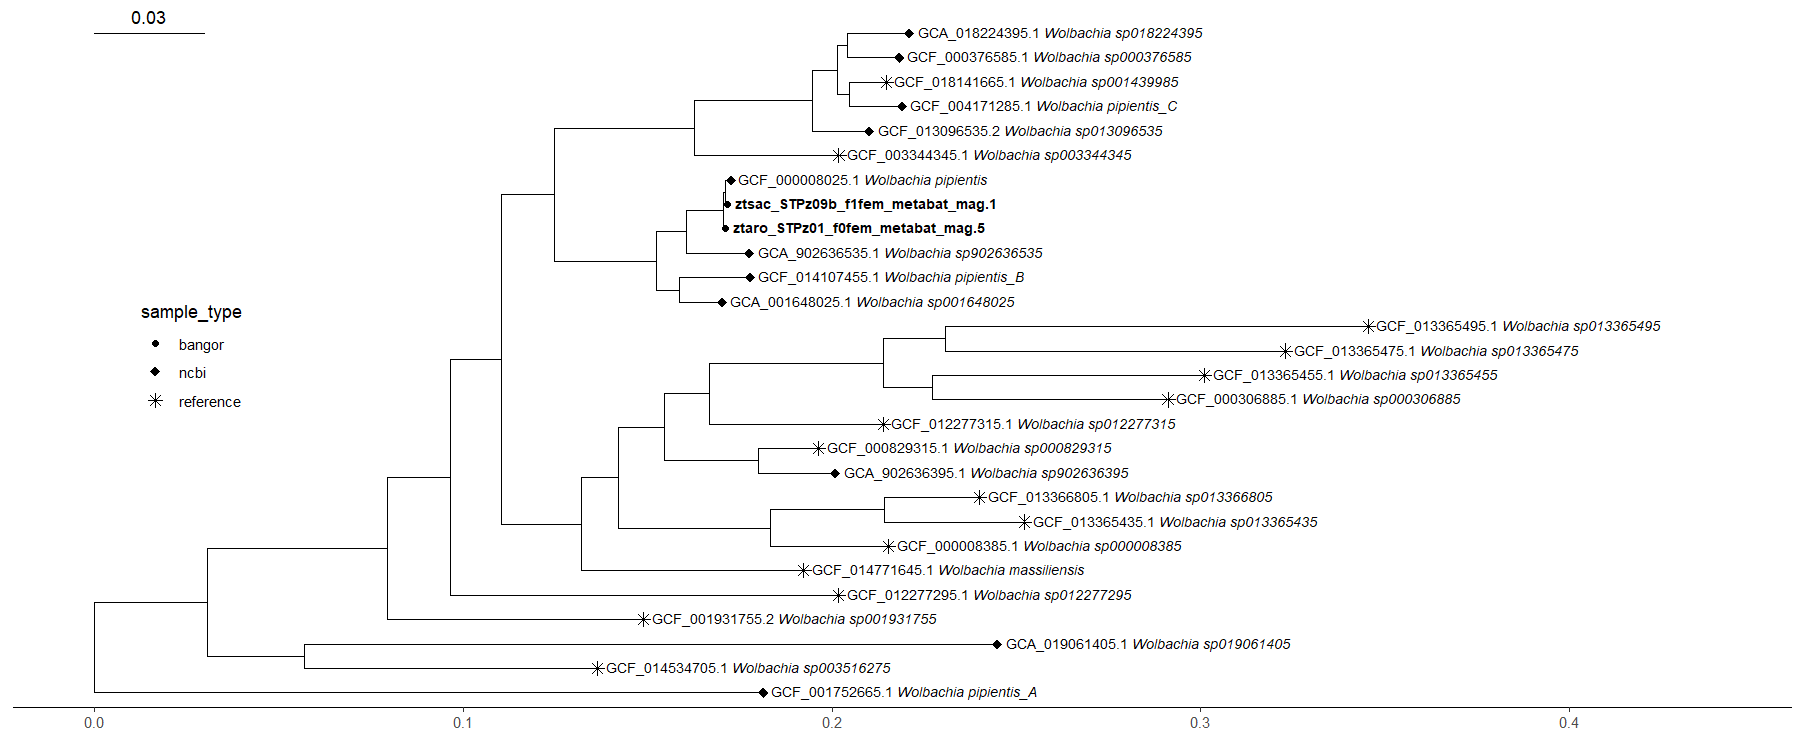
\includegraphics[width=6.01in,height=\textheight,keepaspectratio]{img/Wolbachia_tree.png}

}

\caption{\label{fig-tree}Phylogenetic tree showing which strains of
Wolbachia are closest related to those isolated from Drosophila flies by
Comeault et al.}

\end{figure}%

The tree presents that the closest strain to both of the bangor samples
are \emph{Wolbachia pipentis}.

\subsection{Scripts}\label{scripts-5}

this bit is by no means done, and i need to decide on how i want to do
this bit, do i give a long list of individual files, directories? the
other bits need refinement too, but that can wait until later. £bookmark

\bookmarksetup{startatroot}

\chapter{Flye outputs}\label{flye-outputs}

\section{Introduction}\label{introduction-15}

There were some files outputted from the initial Flye\_asm work done by
Aaron that I thought warranted a look at to sharpen my teeth on.

\section{Methods}\label{methods-11}

\subsection{Flye analysis 1:
assembly\_info.txt}\label{flye-analysis-1-assembly_info.txt}

I created an R script,
\href{https://github.com/tobiasnunn/tnunn_research/blob/aad7006d65994e391c8621132fd7fab3fbf53609/00_scripts/rawflyeanalysis.R}{rawflyeanalysis.R}.
Basic stuff, imports the text files I chose to download (I wonder if I
could download the flye.log files and use a sub() to cut out the
non-useful stuff). This then sorts and processes the data into the table
seen below using a few packages.

\subsection{Flye analysis 2: flye.log}\label{flye-analysis-2-flye.log}

I then went back to the flye.log analysis I wanted to do largely for
posterity. This was horrifyingly complex due to the ``complex'' nature
of the flye.log files. I did this by creating a modified copy of my
assembly\_info.txt file grabber shell script, called
\href{https://github.com/tobiasnunn/tnunn_research/blob/main/Research_Experience_Module/00_scripts/Slurmscripts/flye.loggetter.sh}{flye.loggetter.sh},
using ctrl + h to find and replace instead of manually changing things.
I added this to an existing output directory in my home section of hawk,
which I exported using MobaXterm. This is the folder called
\href{https://github.com/tobiasnunn/tnunn_research/tree/main/Research_Experience_Module/02_middle-analysis_outputs/flyestuff}{flyestuff},
which contains both the flye.log and the assembly\_info.txt files for
each accession, I grouped them as it seemed relevent for organisation
and didnt hinder the coding process at all. The R file I used to
tabulate this is
\href{https://github.com/tobiasnunn/tnunn_research/blob/main/Research_Experience_Module/00_scripts/Rscripts/flyeloganalysis.R}{flyeloganalysis.R}.

\subsection{Results}\label{results-11}

\begin{figure}

\centering{

\begin{table}
\fontsize{12.0pt}{14.4pt}\selectfont
\begin{tabular*}{\linewidth}{@{\extracolsep{\fill}}lrrrr}
\toprule
Accession & Number of contigs & Total length & Largest fragment & Mean fragment length \\ 
\midrule\addlinespace[2.5pt]
3Dt2h & {\cellcolor[HTML]{145CA5}{\textcolor[HTML]{FFFFFF}{166}}} & 3,006,227 & 125,244 & 18,109.80 \\ 
1Dt100g & {\cellcolor[HTML]{1F6DB2}{\textcolor[HTML]{FFFFFF}{153}}} & 2,104,071 & 74,994 & 13,752.10 \\ 
2Dt1e & {\cellcolor[HTML]{2372B6}{\textcolor[HTML]{FFFFFF}{149}}} & 2,332,403 & 70,689 & 15,653.71 \\ 
3Dt1c & {\cellcolor[HTML]{89BEDC}{\textcolor[HTML]{000000}{86}}} & 3,636,266 & 275,317 & 42,282.16 \\ 
3Dt2c & {\cellcolor[HTML]{8DC0DD}{\textcolor[HTML]{000000}{84}}} & 3,819,610 & 247,364 & 45,471.55 \\ 
3Dt2j & {\cellcolor[HTML]{9ECAE1}{\textcolor[HTML]{000000}{75}}} & 2,813,977 & 195,248 & 37,519.69 \\ 
2Dt1l & {\cellcolor[HTML]{E7F1FA}{\textcolor[HTML]{000000}{16}}} & 3,996,506 & 1,089,026 & 249,781.62 \\ 
1Dt2d & {\cellcolor[HTML]{F1F7FD}{\textcolor[HTML]{000000}{6}}} & 5,345,294 & 2,288,975 & 890,882.33 \\ 
1Dt1h & {\cellcolor[HTML]{F3F8FE}{\textcolor[HTML]{000000}{4}}} & 4,336,578 & 2,051,556 & 1,084,144.50 \\ 
1Dt100h & {\cellcolor[HTML]{F5FAFE}{\textcolor[HTML]{000000}{2}}} & 2,379,473 & 2,349,045 & 1,189,736.50 \\ 
\bottomrule
\end{tabular*}
\begin{minipage}{\linewidth}
coverage could not be calculated from this method as no result matched what was found in the \emph{flye.log} files\\
Source: assembly\_info.txt files produced in flye\_asm analysis, August 27th 2024\\
\end{minipage}
\end{table}

}

\caption{\label{fig-assem}Data obtained from flye outputs of samples
taken from the skin microbiome of \emph{Dendrobates tinctorius}}

\end{figure}%

The basic flye output analysis produced this table, as mentioned, I
couldn't get coverage to match what was on the flye.log file that I got
the original of this table from, it is possible that file is the one
that is wrong, but genome coverage is kind of all over the place, so I
just omitted it as I don't think it's one of the mandatory fields. I
chose to sort the table by ``Number of contigs'' rather arbitrarily, but
it does show something interesting in that why is there such a large
range in fragment number?

\begin{figure}

\centering{

\begin{table}
\fontsize{12.0pt}{14.4pt}\selectfont
\begin{tabular*}{\linewidth}{@{\extracolsep{\fill}}lrrrrrr}
\toprule
Accession & Fragments & Total length & Fragments N50 & Largest fragment & Scaffolds & Mean coverage \\ 
\midrule\addlinespace[2.5pt]
3Dt2h & {\cellcolor[HTML]{145CA5}{\textcolor[HTML]{FFFFFF}{166}}} & 3,006,227 & 26,385 & 125,244 & 0 & 390 \\ 
1Dt100g & {\cellcolor[HTML]{1F6DB2}{\textcolor[HTML]{FFFFFF}{153}}} & 2,104,071 & 18,022 & 74,994 & 0 & 318 \\ 
2Dt1e & {\cellcolor[HTML]{2372B6}{\textcolor[HTML]{FFFFFF}{149}}} & 2,332,403 & 22,011 & 70,689 & 0 & 344 \\ 
3Dt1c & {\cellcolor[HTML]{89BEDC}{\textcolor[HTML]{000000}{86}}} & 3,636,266 & 63,365 & 275,317 & 0 & 320 \\ 
3Dt2c & {\cellcolor[HTML]{8DC0DD}{\textcolor[HTML]{000000}{84}}} & 3,819,610 & 69,733 & 247,364 & 0 & 190 \\ 
3Dt2j & {\cellcolor[HTML]{9ECAE1}{\textcolor[HTML]{000000}{75}}} & 2,813,977 & 71,970 & 195,248 & 0 & 350 \\ 
2Dt1l & {\cellcolor[HTML]{E7F1FA}{\textcolor[HTML]{000000}{16}}} & 3,996,506 & 345,773 & 1,089,026 & 0 & 289 \\ 
1Dt2d & {\cellcolor[HTML]{F1F7FD}{\textcolor[HTML]{000000}{6}}} & 5,345,294 & 1,019,507 & 2,288,975 & 0 & 225 \\ 
1Dt1h & {\cellcolor[HTML]{F3F8FE}{\textcolor[HTML]{000000}{4}}} & 4,336,578 & 1,857,409 & 2,051,556 & 0 & 404 \\ 
1Dt100h & {\cellcolor[HTML]{F5FAFE}{\textcolor[HTML]{000000}{2}}} & 2,379,473 & 2,349,045 & 2,349,045 & 0 & 224 \\ 
\bottomrule
\end{tabular*}
\begin{minipage}{\linewidth}
Source: flye.log files produced in flye\_asm analysis, August 27th 2024\\
\end{minipage}
\end{table}

}

\caption{\label{fig-log}Data obtained from flye.log outputs of samples
taken from the skin microbiome of \emph{Dendrobates tinctorius}}

\end{figure}%

This is a table of the type of stuff I first collated in the Summer, it
shares many similarities and cross overs with Table 2, neither have
quality statistics, but both are metadata largely concerning the length
and fragment, a marked difference is this one comes with a concrete
value of coverage. Comparative analysis of them feels like a thing that
would happen in the conclusion to this document.

\subsection{Scripts}\label{scripts-6}

\begin{itemize}
\item
  \href{https://github.com/tobiasnunn/tnunn_research/blob/main/Research_Experience_Module/00_scripts/Slurmscripts/flye.loggetter.sh}{flye.loggetter.sh}
\item
  \href{https://github.com/tobiasnunn/tnunn_research/blob/main/Research_Experience_Module/00_scripts/Rscripts/flyeloganalysis.R}{flyeloganalysis.R}
\end{itemize}

\bookmarksetup{startatroot}

\chapter{Learning, General Progress and Important
Mistakes}\label{sec-genprog}

\section{Evolution of skills}\label{evolution-of-skills}

\subsection{Notebooking with R studio}\label{notebooking-with-r-studio}

I have made much progress with my record-making ability over the course
of the project. When I started, in the summer, I was hardly recording my
actions at all, as I prioritised results over that, assuming it would
not be important later. Then, when the year began I started recording
basic notes in a word document, they were basic and sloppy, but was
better than what came before. Then, at Christmas when I decided to get
my act together and fix errors I had made, I decided I wanted my notes
to be more detailed and meaningful, so I started recording all details
that I felt could be important, dates, exact descriptions, links to
files created and details of what they did and why. These, I did in an R
markdown format, a new concept to me at the time it is essentially an R
document that has more bells and whistles than a traditional R script,
allowing for cross-referencing and text modifications like allowing for
bold and italic text, and the ability to Output to either html or word
depending on what is required.

This was good, but I then discovered that Quarto Markdown existed, from
what I found online it is a direct predecessor to Rmd, so I decided to
make the switch from Notebook 3 onward, this was relatively similar to
Rmd, but it did bring the benefit of a link to zotero for automatic
bibliography (which doesnt work great but its fun it exists, it allows
me to not have to manually make in-line references). And was overall
cleaner with a more updated UI. Then, I discovered R projects. Basically
a way of being able to connect all the scripts to one place for better
linking.

This then developed even further as just recently I discovered R books
existed. They are, as I understand it, a derived kind of R project that
opperates like a book, with the ability to output to html multiple pages
that are all linked together. I decided to make the portfolio an R book
because it's size was monstrous and all of it on 1 long page was ugly. I
still do not understand the full breadth of what this resource can do,
but I have come a long way.

\subsection{Informatic Evolution}\label{informatic-evolution}

The Heatmaps are the main point of the project, and as such I have spent
a lot of time on them. The first version of them was made in the summer
on bacterial samples taken from insect species, including
\emph{Drosophila}. This was made using scripts that were given to me by
Aaron that I adapted largely through a process of trial and error until
I got a good-looking output. When I next attempted it on my own data,
during the prototype, I wanted to do it myself, maybe take aspects of
his code but largely start from scratch, so that is what I did.

The heatmaps went through many different evolutions over time, so many
so that there are details of that process in Notebooks 2, 3 and 4
devoted just to that. I found ways of making better colour schemes,
using API-downloaded metadata to add groupings based on what functions
the pathways had and I added the percentages to the boxes, then fixed
the problem with the axis.

\subsection{Resources}\label{resources}

My library of packages has increased as well. Even before the project I
was confident using ggplot. However, over the course of the project I
have found many packages I have found incredibly useful:

\begin{itemize}
\tightlist
\item
  ggplot - Great for making more detailed / visually appealing visuals
  than base R can accomodate
\item
  Tidyverse (specifically tidyr and deplyr) - these have been very
  useful for data handling and transformation, in too many ways to
  really discuss here, but they allow for greater potential when
  handling data
\item
  gt and flextable - Good for adding style to tables when presenting
  them. They each have benefits and weaknesses, so I cannot recommend
  one over the other
\item
  httr2 - This is the package that allowed me to make API calls to the
  NCBI and KEGG websites, which is the reason I was able to transfer
  large amounts of data as quickly as I did
\end{itemize}

\section{Learning programs}\label{learning-programs}

\subsection{R}\label{r}

My ability to both read and utilize R has increased dramatically from
where I started.

\subsection{bash / slurm}\label{bash-slurm}

I now have a cursery knowledge of how to use these systems on Hawk. I am
not perfect, but I am proficient enough to navigate without issue and
run jobs correctly.

\section{Mistakes}\label{mistakes}

\subsection{Innitial delete}\label{innitial-delete}

All the way back at the beginning of the project, in the summer,
something I did on hawk deleted all of the genomic .fasta files that had
been created by Aaron through Flye-asm. To this day, noone knows exactly
why that happened. However, this did teach me the importance of
understanding something before messing with it and not just racing to
get a result out to be shown. I then took the time to get to grips with
bash and command-line coding by testing on sample documents before
applying commands that ran the risk of modifying the important folders.

(I also then either made copies of all important files from then on or
downloaded them and stored them in OneDrive or Github so they could be
recovered, just in case.)

\section{Next steps}\label{next-steps-1}

\subsection{further analysis}\label{further-analysis}

There are several analyses I did in prototyping that I did not have the
time to do on the final results that I would like to begin the
dissertation with, these include:

\begin{itemize}
\item
  Analysing the significance of the pathways found in the heatmaps
\item
  Analyse the other output files from CheckM2
\item
  making the other heatmap versions (like the cutdown heatmap, the
  ``core'' heatmap, etc)
\item
  figuring out the interactive tree
\item
  get concrete taxonomic assignments somehow, specifically ANI
\end{itemize}

\subsection{Coding languages}\label{coding-languages}

There are a few more languages I would like to learn. Specifically
Python and SQL. I have been thinking about what I would like to do for
my Masters and there are select places that offer Bioinformatics, in the
course of this I learnt about how many tools (including some I have
used, like GTDB-Tk) are created using python and some of the courses
even have researchers make their own tools. This makes me want to have
at least a basic understanding of the language as I now see how it might
be important in conjunction with R (also many internships ask for it as
what i guess is a matter of preference), instead of one or the other. As
I am going to be handling large amounts of data, I believe a smart way
to store and handle it is a SQL server, so that I can make a relational
database and largely do more with the data with less effort. I toyed
with the idea this year, but ultimately decided I did not want to do too
much at one time, and the analyses I was running were too simple to
require it.

\bookmarksetup{startatroot}

\chapter{Conclusion}\label{conclusion-2}

The pathways found in the Chapter~\ref{sec-heatmaps} analysis could be
analysed and lead to a greater understanding of potential functions the
bacteria have in relation to their host, the dyeing poison dart frog. A
potential next step is to test samples from the same taxa of host over
large geographic ranges to see what variation exists between
populations, akin to work done by (\textbf{marzinelli2015?}) , using
public data of known host and sampling site. It has been found that
microbiomes are made of almost universally found or ``core'' symbionts
and more variable microbiota (\textbf{parfrey2018?}). Using public host
data to find these for different taxa could be an interesting avenue of
study. Understanding phylogeny and taxonomy is important for knowing the
variation between samples (\textbf{washburne2018?}). For example, in
this dataset, \emph{Brachybacterium} and \emph{Brevibacterium} are very
closely related, meanng there are fewer differences between them than
the other groups, this means next steps could be to remove the more
distinct samples to bring out those differences. It is important to
inspect the quality of samples before real analysis can be performed,
this is what i used CheckM and CheckM2 for (Chklovski et al. 2023).

I have learnt many skills from this project. My skills using R have
especially grown exponentially from where I started. I have also gained
crucial skills in notebook keeping and organisation that are necessities
for any serious scientist. Secondarily, I have gained skills in
command-line scripting and bash as well as data visualisation. I now
also understand how to use genomic tools such as GTDB-Tk
(\textbf{chaumeil2022?}).

(250 words 5-10 refs, this is split between analysis and skills)

\bookmarksetup{startatroot}

\chapter*{References}\label{references}
\addcontentsline{toc}{chapter}{References}

\markboth{References}{References}

\phantomsection\label{refs}
\begin{CSLReferences}{1}{0}
\bibitem[\citeproctext]{ref-chklovski2023}
Chklovski, Alex, Donovan H. Parks, Ben J. Woodcroft, and Gene W. Tyson.
2023. {``CheckM2: A Rapid, Scalable and Accurate Tool for Assessing
Microbial Genome Quality Using Machine Learning.''} \emph{Nature
Methods} 20 (8): 1203--12.
\url{https://doi.org/10.1038/s41592-023-01940-w}.

\end{CSLReferences}




\end{document}
